\documentclass[a4paper,11pt]{article}
\usepackage{amsmath,amssymb,graphicx,hyperref}
\usepackage[margin=1in]{geometry}
\usepackage{booktabs}
\usepackage{multirow}
\graphicspath{{figures/}}

\title{Geometry--First Cosmology: A Minimal Early Dark Energy Resolution of the $H_0$ and $S_8$ Tensions}
\author{Your Name \\ \textit{Affiliation}}
\date{\today}

\begin{document}

\maketitle

\begin{abstract}
We present a minimal scalar field extension of the Standard Model ($\Lambda$CDM) that simultaneously addresses the Hubble tension ($H_0$) and the clustering tension ($S_8$) through an early-time geometric modification rather than late-time dark sector dynamics. The ``Geometric EDE'' model introduces a scalar field---which we call the Ridder field---with a monodromy-inspired potential containing a narrow shelf at $z \sim 3000$ that briefly contributes a few percent of the total energy density, shrinking the sound horizon $r_s$ and raising the CMB-inferred $H_0$.

Fitting to Planck 2018 + ACT DR6 + pre-DESI BAO + SH0ES data, we find that Geometric EDE with $k = 8$ free parameters achieves $H_0 = 70.6 \pm 0.5$ km s$^{-1}$ Mpc$^{-1}$ and $S_8 = 0.80 \pm 0.01$, reducing the Hubble tension from $4.3\sigma$ to $\sim 2.3\sigma$ and the $S_8$ tension from $2.7\sigma$ to $1.1\sigma$, bringing both into statistical agreement with local and weak-lensing probes. In this baseline configuration, Geometric EDE achieves $\Delta\chi^2 = -10$ relative to $\Lambda$CDM---it fits the data \emph{better}. When DESI Y1 BAO is included, the model converges to a tighter ``convergence window'' with $H_0 \approx 69.5$--$70.5$ km s$^{-1}$ Mpc$^{-1}$ and $r_s \approx 146$--$147$ Mpc, though DESI's preference for a larger sound horizon imposes a $\chi^2$ cost of $\sim +15$--$20$. At equal parameter count, a late-time dynamical model ($w_0 w_a$CDM) modestly improves the fit relative to $\Lambda$CDM ($\Delta\chi^2 \simeq -3$) but leaves both tensions largely intact ($H_0 \simeq 69$, $S_8 \simeq 0.83$). Geometric EDE, by contrast, achieves both better $\chi^2$ (pre-DESI) \emph{and} moves $(H_0, S_8)$ toward the values preferred by local and weak-lensing probes.

Among the $k = 8$ extensions we test, Geometric EDE lies on a Pareto frontier in $(H_0, S_8, \chi^2)$ space: one cannot further improve $H_0$ or $S_8$ without degrading the global fit. At fixed parameter count, geometric early-time changes are statistically preferred over late-time $w_0 w_a$ freedom. The model reduces the sound horizon by $\sim 1\%$ ($\Delta r_s \approx -0.9$ Mpc) and produces a characteristic ``soft shoulder'' in the CMB damping tail---an oscillating residual pattern at the $0.5$--$1.3\%$ level over $600 \lesssim \ell \lesssim 3000$. We show that this signature is consistent with ACT DR6 data and constitutes a concrete falsification target for CMB-S4.

\textbf{Core result:} Within the data sets we study, Geometric EDE is a viable and testable geometric alternative to $\Lambda$CDM that uses two extra degrees of freedom to align early and late probes rather than to over-fit noise. With pre-DESI BAO, the model achieves $\Delta\chi^2 = -10$ (better fit than $\Lambda$CDM) while resolving both tensions. DESI Y1 BAO imposes a $\chi^2$ cost on sound horizon reduction, shifting the interpretation from ``outright victory'' to ``trade-off for tension resolution.'' The predicted damping-tail signature has been confronted with ACT DR6 high-$\ell$ data and remains consistent with current observations; CMB-S4 will provide the decisive test.
\end{abstract}

% =============================================================================
% SECTION I: INTRODUCTION
% =============================================================================

\section{Introduction: From Tensions to Geometry}

\subsection{The Impossible Trinity of Modern Cosmology}

The current cosmological data set contains three pillars that are individually precise but mutually difficult to reconcile. The first is the early universe anchor: Planck 2018 temperature, polarization, and lensing measurements, interpreted in a spatially flat $\Lambda$CDM model, fix the present expansion rate at $H_0 \simeq 67.4 \pm 0.5$ km s$^{-1}$ Mpc$^{-1}$. The same analysis prefers a clustering amplitude often summarized as $S_8 \equiv \sigma_8 \sqrt{\Omega_m/0.3} \simeq 0.83$. These numbers define what we will call the ``Planck corner'' of parameter space and provide a statistically excellent fit to the CMB itself.

The second pillar is the local distance ladder. The SH0ES program, using Cepheid calibrated type Ia supernovae, reports $H_0 = 73.04 \pm 1.04$ km s$^{-1}$ Mpc$^{-1}$, which disagrees with the Planck $\Lambda$CDM value at roughly five standard deviations. This discrepancy, widely known as the Hubble tension, has motivated a large class of extensions to the standard model. More recently, independent JWST calibrations of the Tip of the Red Giant Branch yield $H_0 \approx 70.4 \pm 1.2$ km s$^{-1}$ Mpc$^{-1}$, which sit between Planck and SH0ES and suggest that the true value may lie in a ``middle ground'' around 70 to 71.

The third pillar comes from late time structure growth. Cosmic shear measurements from KiDS, DES, and HSC consistently prefer a lower value of the parameter $S_8$ than the Planck $\Lambda$CDM prediction. A representative example is the DES Year 3 three by two point analysis, which finds $S_8 = 0.776 \pm 0.017$ in $\Lambda$CDM. When summarized in the $(\Omega_m, S_8)$ plane, these weak lensing constraints lie below the Planck contours at the level of roughly two standard deviations. Although this ``clustering tension'' is less dramatic than the Hubble conflict, it is persistent across surveys and analysis pipelines, and it points in the opposite direction from the effect of many proposed Hubble tension solutions.

Taken together, these three results define what we will refer to as an ``impossible trinity.'' $\Lambda$CDM remains an excellent fit to Planck alone, but it struggles to accommodate the combination of CMB, BAO, distance ladder, and large-scale structure measurements in a single parameter region. A model that preserves the simplicity of $\Lambda$CDM at early times tends to track the Planck value of $H_0$ and inherit its high $S_8$, which sits in tension with both local distance ladder and weak lensing data. A model that raises $H_0$ toward the SH0ES value by altering the late time equation of state often worsens the fit to BAO and supernovae or pushes $S_8$ even higher. Conversely, models that reduce $S_8$ through modified gravity or strong dark sector interactions can be difficult to reconcile with the CMB and with bounds on fifth forces. Almost all existing proposals relieve one leg of the trinity at the expense of another, creating a ``cosmological see-saw'' effect. In what follows we adopt a complementary perspective and ask whether a controlled geometric modification of the pre recombination expansion history can move all three probes toward concordance without paying a prohibitive cost in goodness of fit.

\begin{figure}[ht]
\centering

\includegraphics[width=0.85\textwidth]{paper_tension_reduction.png}
\caption{Quantifying the cosmological tensions and their resolution. \textbf{Left:} The Hubble tension, expressed as the discrepancy between $\Lambda$CDM (Planck) and the SH0ES Cepheid measurement, is reduced from $4.3\sigma$ to $\sim 2.3\sigma$ by Geometric EDE. \textbf{Right:} The clustering tension between Planck and DES Y3 weak lensing is reduced from $2.7\sigma$ to $1.1\sigma$. Geometric EDE achieves simultaneous improvement on both fronts---a result that most other extensions struggle to deliver.}
\label{fig:tension_reduction}
\end{figure}

\subsection{The New Data Landscape: JWST and DESI}

The observational landscape that motivated the original Hubble tension is not the one we live in now. Over the last two years, JWST and DESI have begun to reshape both ends of the distance ladder, and any proposal to resolve the tensions has to be framed against this evolving backdrop. In this subsection we summarize the pieces that matter most for our geometry--first approach.

JWST has sharpened the local side of the problem. Using JWST near--infrared imaging of Tip of the Red Giant Branch (TRGB) and JAGB stars, the Chicago--Carnegie Hubble Program now finds a Hubble constant of $H_0 = 70.39 \pm 1.22$ km s$^{-1}$ Mpc$^{-1}$, squarely between the Planck--$\Lambda$CDM value and the original SH0ES result. This intermediate value suggests that at least part of the earlier binary picture---Planck at 67 and SH0ES at 73---was shaped by systematics that are now being tamed by better data. At the same time, new JWST Cepheid observations have re-examined one of the main proposed systematics on the SH0ES side, namely crowding and blending in HST images. These studies find no evidence for a large bias that would drive the Cepheid ladder down to the Planck value, so the high end of the ladder remains statistically viable once measurement errors are properly propagated. Taken together, the TRGB and Cepheid programs point away from a simple ``one experiment is wrong'' narrative and toward a genuine intermediate scale, $H_0 \sim 70$--$71$ km s$^{-1}$ Mpc$^{-1}$, that future local probes are converging toward.

On the intermediate and high--redshift side, DESI Year 1 BAO results have introduced a different kind of challenge for $\Lambda$CDM. Because BAO measurements constrain relative distances, DESI Phase I does not by itself determine an absolute $H_0$; an external calibrator is still required. However, when combined with CMB data, the DESI collaboration finds a preference for dynamical dark energy---with $w_0 > -1$ and $w_a < 0$---over a rigid cosmological constant at roughly the $2.5$--$4\sigma$ level, depending on the exact data combination. This preference does not appear as a dramatic failure in any single observable; rather, it shows up as a mismatch in how the standard ruler, set by the sound horizon $r_s$ at the drag epoch, projects onto low--redshift distance and expansion data. The DESI results are therefore not a direct arbiter of the $H_0$ tension, but they strongly favor departures from a constant $\Lambda$, indicating a dark energy history that invites extensions like Geometric EDE rather than the simplest constant-$\Lambda$ picture.

Follow-up analyses have sharpened this point in the direction most relevant for our work. Jiang and collaborators have argued that the DESI preference for non-$\Lambda$ behavior is naturally explained in models where the pre-recombination sound horizon is modified, as in Early Dark Energy scenarios, rather than by invoking a highly contrived late--time equation of state. Independent re-analyses by Wang and others reach similar conclusions: once one allows for mild departures from $\Lambda$CDM, the combined CMB+BAO data tend to favor evolving dark energy over a pure cosmological constant, and the preferred region in parameter space overlaps with those EDE models that rescale $r_s$ while keeping low--redshift distances under control. These results do not yet single out a unique mechanism, but they do shift the burden of proof. A model that leaves $r_s$ untouched and tries to repair everything at $z < 2$ has to work against the direction in which DESI is nudging the data.

Putting the JWST and DESI pieces together, a new ``convergence window'' begins to emerge. Local probes anchored by JWST now cluster around $H_0 \approx 70$--$71$ rather than 73, while early- and mid-redshift probes increasingly favor some form of dynamical dark energy or early-time modification that changes $r_s H_0$ without wrecking the fit to the CMB. The tensions are not gone, but their geometry has changed: instead of a binary clash between ``Planck 67'' and ``SH0ES 73,'' the data seem to be drifting toward an intermediate expansion rate and away from a strictly rigid dark energy sector. In the rest of this paper we interpret our scalar--field construction precisely in that context, asking whether a minimal early--time modification of the geometry can land naturally in this JWST/DESI window while also addressing the persistent discrepancy in $S_8$.

\subsection{A Geometry--First Strategy}

Our starting point is not a new fluid or a hidden sector, but the geometry itself. The Hubble constant and the clustering amplitude are encoded in how the scale factor evolves and in how distances project on to observables, so we ask a simple question. Instead of postulating new, poorly constrained interactions, we ask what minimal change in the expansion history the data will tolerate that can ease both the $H_0$ and $S_8$ tensions at once. The logic is to let the data pull on the metric and then read off which parts of the expansion history actually need to move.

To implement this idea we begin with the Chevallier--Polarski--Linder equation of state, treated not as a fundamental model but as a diagnostic tool. CPL supplies two free parameters, $w_0$ and $w_a$, which allow the late--time dark energy sector to deviate smoothly from a cosmological constant across $0 \lesssim z \lesssim 2$. By fitting CPL to Planck, BAO, and local $H_0$ information in a common likelihood, we can test a clean hypothesis: that a flexible but otherwise standard dark energy fluid at late times is enough to reconcile the tensions. If the CPL posterior keeps $w(z)$ very close to $-1$ while still leaving $H_0$ and $S_8$ in conflict, then late--time freedom is not the direction the data are asking us to move. In that case, we are naturally pushed to look earlier in the thermal history.

Our exploration chains confirm this expectation. The CPL model achieves $\Delta\chi^2 = -3.3$ relative to $\Lambda$CDM (a genuine improvement in fit) but lands at $H_0 = 69.17$ and $S_8 = 0.828$---leaving both tensions largely intact. Late-time freedom alone is not sufficient to move the posteriors into the region preferred by local and weak-lensing probes. This distinction is crucial: unlike phenomenological late-time approaches (CPL, $w_0 w_a$) that modify dark energy evolution at $z < 2$, Geometric EDE operates as Early Dark Energy, active during the pre-recombination era. This allows modification of the sound horizon---the key to resolving the Hubble tension---rather than simply improving late-time expansion history fits.

Once late--time dynamics have been used in this way and found wanting, a geometry--first strategy turns to the pre--recombination era. At those redshifts the key quantity is the sound horizon $r_s$, which sets the physical scale for both the acoustic peaks in the CMB and the BAO feature in the galaxy distribution. Changing $r_s$ while keeping the acoustic angles fixed shifts the inferred value of $H_0$ without directly tampering with the distance ladder, and it can also modify the growth history that feeds into $S_8$. In the rest of the paper we therefore focus on minimal scalar field configurations that introduce a narrow, percent--level modification to the early expansion rate, adjust $r_s$ accordingly, and then relax into a conventional late--time tail, so that the geometry rather than an exotic dark sector carries the burden of resolving the tensions.

\subsection{Our Proposal: Geometric EDE ($\phi$CDM)}

Our proposal is to take the geometric hint from the data at face value and implement it with the smallest possible new ingredient. We introduce a single scalar field, $\phi$---which we call the Ridder field purely as a label; nothing in the analysis depends on that name---evolving in a monodromy--inspired potential that has three regimes along its trajectory: a high plateau in the early universe, a narrow shelf at intermediate redshift, and a shallow tail at late times. As the field rolls, it briefly slows near the shelf around $z \sim 3000$, where it contributes a percent--level fraction of the total energy density and temporarily accelerates the pre--recombination expansion. This short episode of early dark energy shrinks the sound horizon $r_s$ and therefore shifts the inferred Hubble constant upward when the CMB and BAO are fit together. After the shelf, the field continues into a slowly varying tail that behaves like a mildly dynamical dark energy component and can track the broad trends in the $w(z)$ reconstructions favored by DESI.

In the main analysis we keep the couplings of $\phi$ as simple as possible. The field is taken to interact only through gravity, with no direct coupling to dark matter or other species. There is therefore no long--range fifth force at late times and no need to hide new interactions from existing constraints. The only freedom the model uses is encoded in the shape of the potential and in the timing and height of the early shelf, which are parameterized in a way that maps directly onto the evolution of the background metric. This is why we refer to the scenario as ``Geometric EDE'' or $\phi$CDM: it relieves the tensions by changing the geometry of the expansion history rather than by introducing a new dark fluid with an arbitrary equation of state.

When this Geometric EDE model is fit on the same likelihoods and with the same nuisance treatment as $\Lambda$CDM and CPL, a clear qualitative pattern emerges. The early shelf lifts the inferred Hubble constant toward the overlap region suggested by JWST--calibrated TRGB measurements and the higher end of the local distance ladder, while the modified growth history pulls the clustering amplitude $S_8$ closer to the values preferred by weak--lensing surveys. Specifically, our production MCMC runs with pre-DESI BAO achieve:

\begin{itemize}
    \item $H_0 = 70.62 \pm 0.48$ km s$^{-1}$ Mpc$^{-1}$ (vs.\ $68.29 \pm 0.38$ for $\Lambda$CDM)
    \item $S_8 = 0.798 \pm 0.010$ (vs.\ $0.825 \pm 0.007$ for $\Lambda$CDM)
    \item $\Delta\chi^2 = -10.1$ relative to $\Lambda$CDM (i.e., EDE fits the data \emph{better})
\end{itemize}

When DESI Y1 BAO is added, the picture evolves. DESI's precise BAO measurements prefer a sound horizon close to the $\Lambda$CDM value ($r_s \approx 147$--$148$ Mpc), which creates tension with EDE's reduced sound horizon ($r_s \approx 146$ Mpc). In our Tier 5 analysis incorporating DESI (Table~\ref{tab:tier5_running}), EDE pays a $\chi^2$ cost of $\sim +15$--$20$ relative to $\Lambda$CDM to reach the convergence window. The model still delivers higher $H_0$ ($\approx 69.9$ km s$^{-1}$ Mpc$^{-1}$) and lower $S_8$ ($\approx 0.81$), but the interpretation shifts from ``EDE wins on all metrics'' to ``EDE trades $\chi^2$ for tension resolution.'' Critically, the predicted ``soft shoulder'' signature in the CMB damping tail---an oscillating residual pattern at the $\sim 1\%$ level---is shown to be consistent with ACT DR6 high-$\ell$ data. In the sections that follow we quantify these statements, show how the best--fit Geometric EDE solutions lie on a Pareto front in the $(H_0, S_8, \chi^2)$ space, and confront the predicted damping-tail signature directly with ACT observations.

\subsection{Outline of the Paper}

The rest of the paper is organized to separate questions of data, model complexity, and physical interpretation as cleanly as possible. In Section II we begin with a precise definition of the Ridder field as an effective fluid, specifying its energy budget in terms of a shelf and tail contribution; we then describe the data sets and likelihoods used in our analysis, including both Planck 2018 and ACT DR6 CMB data, and we define three observational ``worlds,'' each built around the same CMB backbone with different local $H_0$ anchors. This lets us ask how the models behave with and without explicit late--time priors while keeping the high--redshift information fixed.

Section III introduces the three cosmological models we compare: the Standard Model $\Lambda$CDM, a late--time dynamical dark energy model of the Chevallier--Polarski--Linder form ($w_0 w_a$CDM), and the Geometric EDE ($\phi$CDM) model described above. We spell out the parameter counting, explain the ``parameter diet'' that keeps Geometric EDE at the same effective dimensionality as CPL, and define the derived diagnostics such as $H_0$, $S_8$, and $r_s H_0$ that we use throughout.

Section IV describes the statistical methods: the MCMC setup and convergence criteria, the definition of $\chi^2_{\rm post}$ (posterior deviance) that we use throughout, and the Pareto front construction that summarizes trade--offs between fit quality, $H_0$, and $S_8$. We also explain the AIC and BIC comparisons with particular attention to the equal--$k$ comparison between CPL and Geometric EDE.

Section V presents the core numerical results, comparing models at fixed parameter count within each observational world. We report posterior constraints on $H_0$ and $S_8$ and show how Geometric EDE simultaneously raises $H_0$, lowers $S_8$, and improves $\chi^2$ relative to both $\Lambda$CDM and CPL. We also present extended results incorporating DESI Y1 BAO and DES Y1 weak lensing (the ``Growth World''), showing that the model converges to a narrow ``convergence window'' with $H_0 \approx 70$--$70.5$ km s$^{-1}$ Mpc$^{-1}$.

Section VI focuses on physical interpretation and observational signatures. We examine how the Geometric EDE solutions move the cosmological posteriors in the $(H_0, S_8)$ plane and identify the regions of parameter space that resolve both tensions. Critically, we present a direct test of the predicted ``soft shoulder'' in the CMB damping tail using ACT DR6 high-$\ell$ data, showing that the characteristic oscillating residual pattern at the $\sim 1\%$ level is consistent with current observations and constitutes a falsification target for CMB-S4.

In Section VII we discuss the monodromy motivation for the unified Ridder potential that underlies our implementation of $\phi$CDM. We show how the plateau, shelf, and tail structure arises from a standard axion monodromy template, and we check that the required masses, energy scales, and field excursions sit in the same regime as existing monodromy inflation and quintessence models. Section VIII collects robustness tests and connections to the recent JWST and DESI results, including variations in data combinations and exploratory runs with additional freedom in the scalar sector.

Finally, Section IX summarizes our findings and outlines the observational prospects. We emphasize how a geometry--first early dark energy shelf can sit within the emerging $H_0 \sim 70$--$71$ ``convergence window,'' how it compares to late--time dynamical solutions in both fit quality and information criteria, and how the ACT-validated damping-tail signature provides a concrete path to confirmation or falsification with forthcoming CMB surveys.

% =============================================================================
% SECTION II: DATA SETS, LIKELIHOODS, AND WORLDS
% =============================================================================

\section{Data and Likelihoods: Building Fair ``Worlds''}

% -----------------------------------------------------------------------------
% II.1 THE RIDDER FIELD AS AN EFFECTIVE FLUID
% -----------------------------------------------------------------------------

\subsection{The Ridder Field as an Effective Fluid}
\label{sec:ridder_fluid}

We treat the Ridder field as an additional component in the background expansion, on top of the usual radiation, matter, and cosmological constant of $\Lambda$CDM. Rather than starting from a specific ultraviolet completion, we work with an effective fractional energy density history, $\Omega_\phi(a)$, that captures two features of interest. At early times the field produces a localized ``shelf'' of extra energy density around $z \sim 3000$, and at late times it approaches a smooth tail that mimics dark energy.

At the homogeneous level we write the total energy budget as
\begin{equation}
\Omega_{\rm tot}(a) = \Omega_r(a) + \Omega_m(a) + \Omega_\Lambda(a) + \Omega_\phi(a),
\end{equation}
with $\Omega_r$, $\Omega_m$, and $\Omega_\Lambda$ as in $\Lambda$CDM. The Ridder contribution is specified by
\begin{equation}
\Omega_\phi(a) = \Omega_{\rm shelf}(a) + \Omega_{\rm tail}(a).
\end{equation}
The shelf is modeled as a lognormal bump in scale factor,
\begin{equation}
\Omega_{\rm shelf}(a) = f_{\rm shelf} \, \Omega_{\rm tot}(a_c) \, \exp\!\left[ -\frac{(\ln a - \ln a_c)^2}{2\sigma_{\ln a}^2} \right],
\end{equation}
where $a_c$ sets the time of the shelf, $\sigma_{\ln a}$ its width in $\ln a$, and $f_{\rm shelf}$ the peak fractional contribution at $a = a_c$. In the minimal model used in this work we fix $a_c$ and $\sigma_{\ln a}$ to the values calibrated in our Tier-10 analysis and treat $f_{\rm shelf}$ as the single new amplitude parameter controlling the size of the modification to the sound horizon.

The late-time tail is described by an effective equation of state $w_{\rm tail}(a)$, chosen so that the field interpolates smoothly from the shelf regime into a dark-energy like component at $z \lesssim 1$. For the runs presented here we use a simple constant equation of state,
\begin{equation}
w_{\rm tail} = w_0,
\end{equation}
with $w_0$ fixed close to $-1$ so that the tail tracks the behavior of a cosmological constant at late times. The corresponding energy density scales as
\begin{equation}
\rho_{\rm tail}(a) \propto a^{-3(1+w_0)}.
\end{equation}
This construction keeps the number of free parameters minimal while still capturing the two essential features of the Ridder field: a localized early-time shelf that shrinks $r_s$ at recombination and a smooth late-time tail that contributes to cosmic acceleration.

In the perturbation sector we treat the Ridder component as a smooth fluid with sound speed $c_s^2 \approx 1$, following the standard implementation of scalar-field dark energy in Boltzmann codes. This choice reproduces the behavior of a light canonical scalar with sub-horizon fluctuations suppressed and ensures that the primary signatures of the model arise through geometry and small shifts in the acoustic peak structure rather than from new clustering physics at late times. We set the direct coupling between the field and dark matter to zero ($\beta = 0$) in all Tier-5 and Tier-10 runs, so that the Ridder field influences observables only through its contribution to the background and to metric perturbations.

Although we work with this effective fluid description in the data analysis, it is useful to keep in mind the scalar-field picture that motivates it. A canonical field $\phi$ with Lagrangian
\begin{equation}
\mathcal{L}_\phi = -\tfrac{1}{2}(\partial\phi)^2 - V(\phi)
\end{equation}
and a structured potential $V(\phi)$ that contains a shallow plateau followed by a monodromy-like tail naturally produces the shelf-plus-tail pattern encoded in $\Omega_\phi(a)$. In such models the field remains frozen at early times, briefly contributes a finite fraction of the total energy density as it rolls across the plateau around $z \sim 3000$, and then relaxes slowly along the tail, sourcing late-time acceleration. In this paper we work directly with the effective $\Omega_\phi(a)$ and $w(a)$ implied by this class of potentials and leave a detailed microphysical mapping of $\{f_{\rm shelf}, a_c, \sigma_{\ln a}, w_0\}$ to specific choices of $V(\phi)$ to future work.

In this sense the Ridder field provides an explicit example of a dark-sector degree of freedom that is dynamically active at recombination and still evolving today, which we return to in the discussion of coincidence and thermal history in Section~\ref{sec:outlook}.

% -----------------------------------------------------------------------------
% II.2 CMB DATA - PLANCK + ACT VERSION (ACTIVE)
% -----------------------------------------------------------------------------

\subsection{CMB Data (Planck 2018 + ACT DR6)}
\label{sec:cmb_data}

Our high--redshift constraints come from a combined Planck 2018 and ACT DR6 analysis. Planck provides all--sky coverage and exquisite control of large and intermediate angular scales, while ACT sharpens the view of the damping tail at high multipoles ($\ell \gtrsim 600$). Taken together they define the early--universe baseline against which we test $\Lambda$CDM, CPL, and Geometric EDE.

For Planck we adopt the standard 2018 likelihood combination used in cosmological parameter studies. This includes the high--$\ell$ TT, TE, and EE spectra, the low--$\ell$ temperature likelihood, the low--$\ell$ polarization likelihood, and the four--point lensing reconstruction. High--$\ell$ information is supplied by the Plik--type likelihood, while the largest angular scales are modeled by the Commander temperature and SimAll polarization likelihoods. We retain the full set of Planck nuisance parameters and marginalize over them identically for each cosmological model so that differences in $\chi^2$ arise from changes in the expansion history rather than from a different foreground treatment.

ACT DR6 contributes independent high--resolution measurements of the CMB power spectra on smaller angular scales. We use the DR6 TT, TE, and EE bandpowers over the multipole range $600 \lesssim \ell \lesssim 3000$ together with the accompanying covariance matrices and foreground model supplied by the ACT collaboration. The ACT likelihood includes approximately 20 nuisance parameters describing Galactic and extragalactic foregrounds (thermal and kinetic SZ, CIB, radio point sources) as well as calibration factors for each frequency channel. These nuisances are sampled jointly with the cosmological parameters.

The ACT likelihood is treated as statistically independent from Planck and is simply multiplied into the joint posterior. Where nuisance parameters overlap in physical content, such as foreground amplitudes, we follow the published prescriptions of the Planck and ACT teams rather than introducing new shared templates. This keeps the combination conservative and avoids extracting information from detailed cross--calibration.

In all of the ``worlds'' defined below, the baseline CMB block consists of the full Planck 2018 likelihood plus the ACT DR6 spectra, with the same multipole ranges, masks, and nuisance priors applied regardless of whether the cosmology is $\Lambda$CDM, CPL, or Geometric EDE. Lensing from Planck is included unless explicitly stated, while ACT lensing is not yet folded into the main likelihood. This common CMB backbone ensures that every comparison in Sections IV--VI is made on a fair footing, and that any improvement or degradation in fit quality reflects real differences in the geometric history rather than changes in the underlying microwave data. Critically, the ACT high--$\ell$ data provide direct sensitivity to the ``soft shoulder'' signature predicted by Geometric EDE in the damping tail (Section~\ref{sec:cmb_residuals}).

% -----------------------------------------------------------------------------
% II.1 CMB DATA - PLANCK ONLY VERSION (ARCHIVED)
% (Use this version if NOT including ACT DR6)
% -----------------------------------------------------------------------------

% \subsection{CMB Data (Planck 2018)}
% \label{sec:cmb_planck}
%
% Our primary high--redshift anchor is the Planck 2018 temperature and polarization data set. Throughout this work we use the baseline Planck likelihood combination recommended for cosmological parameter estimation. This includes the high--multipole TT, TE, and EE spectra, the low--$\ell$ temperature likelihood, the low--$\ell$ polarization likelihood, and the four--point reconstruction of the lensing potential. Together, these provide tight constraints on the acoustic peak structure, the damping tail, and the integrated growth of structure.
%
% In practice, the high--$\ell$ TT, TE, and EE information enters through the Plik--type likelihood, while the largest angular scales are described by the Commander temperature likelihood and the SimAll low--$\ell$ polarization likelihood. The CMB lensing likelihood is built from the reconstructed convergence power spectrum and is included in all of our ``worlds'' unless stated otherwise. We retain the full set of Planck nuisance parameters and marginalize over them in exactly the same way for every model, so that any change in fit quality can be traced to the cosmological sector rather than to a different treatment of foregrounds or calibration.
%
% Because our goal is to compare $\Lambda$CDM, CPL, and Geometric EDE on equal footing, each model is run against the same Planck likelihood combination with identical data cuts and priors. The Planck CMB block therefore serves as the common backbone for all the data combinations we consider. ACT DR6 and other small--scale CMB experiments provide valuable independent checks on high--$\ell$ structure, but a full joint treatment lies beyond the scope of this initial analysis. Where relevant, we comment on how our preferred solutions sit relative to published ACT and SPT constraints, while keeping the formal likelihood analysis anchored in the Planck 2018 data set.

% -----------------------------------------------------------------------------
% II.3 LOW-REDSHIFT PROBES
% -----------------------------------------------------------------------------

\subsection{Low--Redshift Probes}
\label{sec:lowz}

To connect the early--time CMB constraints to the late--time expansion and growth history, we supplement the microwave data with a standard set of low--redshift probes. These measurements determine how distances and structure formation respond to different choices of expansion history, and they are included in an identical way for $\Lambda$CDM, $w_0 w_a$CDM, and Geometric EDE ($\phi$CDM). This ensures that any change in $\chi^2$, $H_0$, or $S_8$ can be traced to the cosmological model rather than to differences in the data or likelihood treatment.

For baryon acoustic oscillations we use the pre--DESI BAO compilation employed in our production chains. This includes distance and Hubble rate constraints from BOSS and eBOSS galaxy samples, together with the 6dFGS and SDSS Main Galaxy Sample measurements at low redshift. In practice we work with the published compressed BAO likelihoods in terms of $D_M(z)$, $H(z)$, and the sound horizon $r_s$, with covariance matrices supplied by the survey teams. These BAO points anchor the expansion at intermediate redshifts and are crucial for diagnosing whether a given model is adjusting the sound horizon at recombination or reshaping $H(z)$ at late times.

For supernovae we include the Pantheon+ Type Ia compilation as a luminosity distance ladder. In the main analysis the choice of supernova sample and its nuisance parameter treatment is held fixed across all models, so the supernovae act only as a common constraint linking the CMB+BAO geometry to the low--redshift distance scale. We marginalize over the absolute magnitude and other standard nuisance parameters, so that the supernovae do not impose an independent $H_0$ prior but instead calibrate the relative shape of the Hubble diagram.

Local measurements of the Hubble constant enter through explicit priors. We consider two such anchors that represent the current state of the distance ladder. The first is the SH0ES Cepheid--calibrated supernova determination, which favors a relatively high value of the Hubble constant and has been the main driver of the original Hubble tension. The second is the JWST--enabled TRGB calibration from the Chicago--Carnegie Hubble Program, which uses Tip of the Red Giant Branch and related standard candles to obtain a value of $H_0$ in the emerging middle ground around $70$ to $71$ km s$^{-1}$ Mpc$^{-1}$. In our likelihood, these enter as Gaussian priors on $H_0$ with means and variances taken from the respective analyses. By toggling these priors on and off we can study how each model behaves when conditioned on no local anchor, a high SH0ES anchor, or a TRGB/JWST anchor that already points toward the geometric solution.

The combination of CMB, BAO, supernovae, and local $H_0$ priors defines the low--redshift structure of each ``world'' we analyze. The next subsection formalizes these worlds and clarifies how we use them to separate questions about early geometry from questions about late--time calibration.

% -----------------------------------------------------------------------------
% II.4 DEFINING THE THREE WORLDS
% -----------------------------------------------------------------------------

\subsection{Defining the Three ``Worlds''}
\label{sec:worlds}

To keep the analysis transparent, we organize all our runs into three benchmark ``worlds.'' Each world uses the same CMB block described in Section II.1 and the same BAO and supernova likelihoods described above, but differs in how the late--time Hubble scale is anchored. This division lets us ask a clean set of questions: what does each model do when we do not tell it anything about the local $H_0$, what does it do when we insist on the SH0ES value, and what happens when we calibrate instead with the TRGB/JWST middle ground.

The \textbf{Base world} consists of Planck 2018 (plus ACT DR6 if included), the pre--DESI BAO set, and the supernova compilation, with no explicit local $H_0$ prior. In this world the Hubble constant is inferred indirectly through the combination of early--time geometry and low--redshift distance ratios. It is the natural arena in which to test whether the data themselves, absent any late--time anchor, already prefer a departure from $\Lambda$CDM when given the option of CPL or Geometric EDE. It also clarifies whether the early shelf in $\phi$CDM is being driven purely by the SH0ES prior or has independent support from the CMB+BAO combination.

The \textbf{SH0ES world} adds a Gaussian prior $H_0 = 73.04 \pm 1.04$ km s$^{-1}$ Mpc$^{-1}$ to the Base combination. This world represents the traditional Hubble tension setup in which Planck and BAO are asked to coexist with a higher local Hubble constant. In this setting $\Lambda$CDM typically pays the price in $\chi^2$, and CPL can harvest some improvement by flexing the late--time equation of state while leaving $r_s$ unchanged. Our goal here is to test whether Geometric EDE can do better, by reshaping the pre--recombination geometry to raise $H_0$ while simultaneously lowering $S_8$, and to quantify exactly how much $\chi^2$ it must pay relative to both $\Lambda$CDM and CPL at equal parameter count.

The \textbf{TRGB world} instead augments the Base combination with a Gaussian prior $H_0 = 69.8 \pm 1.7$ km s$^{-1}$ Mpc$^{-1}$ from JWST--calibrated TRGB measurements. In this world the local anchor already lies near the value that Geometric EDE tends to produce when the shelf is tuned to relieve the tension. This allows us to check robustness in the opposite direction: if we remove the high SH0ES pull and replace it with an intermediate anchor, does $\phi$CDM naturally settle into the same geometry, or does it rely on the extreme end of the distance ladder to justify its shelf. The TRGB world also provides a clean setting in which to compare the late--time tail of the potential to DESI's preferred $w(z)$ reconstructions, since it does not force the model to chase an outlying $H_0$.

Throughout the paper we emphasize that these worlds are not different theories but different posterior slices of the same models under different late--time conditions. Each world applies the same data and nuisance treatment across $\Lambda$CDM, CPL, and Geometric EDE. This structure makes it straightforward to present normalized $\Delta\chi^2$, AIC, and BIC comparisons in Section IV and to interpret the movement of $H_0$ and $S_8$ across worlds as genuine geometric responses rather than artifacts of an inconsistent likelihood setup.

% -----------------------------------------------------------------------------
% II.5 LIKELIHOOD PIPELINE AND NUISANCE PARAMETERS
% -----------------------------------------------------------------------------

\subsection{Likelihood Pipeline and Nuisance Parameters}
\label{sec:pipeline}

\paragraph{Sampling Framework.}
All parameter estimation is performed using the Cobaya MCMC sampler, which interfaces with a modified version of the CLASS Boltzmann code that includes our Geometric EDE implementation. The same likelihood modules, nuisance parameter treatments, and sampling settings are applied identically to $\Lambda$CDM, $w_0 w_a$CDM, and $\phi$CDM, ensuring that any differences in posterior distributions arise solely from the cosmological model rather than from analysis choices.

\paragraph{Likelihoods.}
We use the three data combinations defined in Section~II.3: the Base world (Planck 2018 + ACT DR6 + pre-DESI BAO), the SH0ES world (Base + Cepheid prior), and the TRGB world (Base + JWST/TRGB prior). Our extended Tier 5 analysis additionally incorporates DESI Y1 BAO and DES Y1 weak lensing (the ``Growth World''). All likelihoods are implemented through standard Cobaya modules and applied identically to $\Lambda$CDM, CPL, and Geometric EDE.

\paragraph{Nuisance Parameters.}
The Planck likelihoods include standard nuisance parameters for instrumental calibration, beam uncertainties, and foreground contamination. These parameters are sampled jointly with the cosmological parameters and are assigned identical priors across all three models. For the plik\_lite likelihood, foreground and calibration nuisances are marginalized analytically, reducing the dimensionality of the sampling problem while preserving consistency across model comparisons. No additional nuisance parameters are introduced for the Geometric EDE model beyond those required by the Planck likelihood. The EDE sector parameters ($\log_{10}a_c$, $\Lambda_{\rm EDE}$) enter only through their effect on the background and perturbation evolution and do not couple to instrumental or astrophysical systematics.

\paragraph{Convergence and Model Comparison.}
Full details of the MCMC convergence criteria (Gelman--Rubin $R - 1 < 0.01$, $N \geq 1000$ samples per chain) and information--theoretic model comparison (AIC, BIC) are given in Section~IV. The key point here is that all three models are run through the same Cobaya+CLASS pipeline with identical stopping criteria and model comparison metrics.

% -----------------------------------------------------------------------------
% II.6 FAIRNESS CHECKLIST
% -----------------------------------------------------------------------------

\subsection{Summary: The Fairness Checklist}
\label{sec:fairness}

To ensure a fair comparison across models, the following elements are held \emph{identical} for $\Lambda$CDM, $w_0 w_a$CDM, and Geometric EDE ($\phi$CDM):

\begin{itemize}
    \item \textbf{Data:} Same likelihood modules (Planck 2018, BAO, lensing) and same local $H_0$ priors defining each world.
    \item \textbf{Nuisances:} Same foreground and calibration parameters with identical priors.
    \item \textbf{Sampler:} Same MCMC engine (Cobaya), stopping criteria ($R - 1 < 0.01$), and convergence checks ($N \geq 1000$ per chain).
    \item \textbf{Reference:} All $\Delta\chi^2$, $\Delta$AIC, and $\Delta$BIC values reported relative to the best--fit $\Lambda$CDM point within each data combination.
\end{itemize}

Any difference in fit quality therefore reflects the cosmological model, not the analysis pipeline.

% =============================================================================
% SECTION III: MODELS AND PARAMETER COUNTING
% =============================================================================

\section{Models and Parameter Counting}

% -----------------------------------------------------------------------------
% III.1 STANDARD MODEL: ΛCDM
% -----------------------------------------------------------------------------

\subsection{Standard Model: $\Lambda$CDM}
\label{sec:lcdm}

We begin with the usual six--parameter $\Lambda$CDM model, which serves as the reference point for all comparisons in this work. The base parameter set is
\begin{equation}
\{\omega_b, \omega_c, \theta_s, \tau, n_s, \ln(10^{10} A_s)\},
\end{equation}
where $\omega_b$ and $\omega_c$ are the physical baryon and cold dark matter densities, $\theta_s$ is the angular size of the sound horizon at recombination, $\tau$ is the optical depth to reionization, and $n_s$ and $A_s$ describe the primordial scalar power spectrum. These six parameters are sampled with the same priors and numerical settings in all three worlds defined in Section II.3, and all nuisance parameters associated with Planck, BAO, and supernova data are treated identically across every model. This makes $\Lambda$CDM the clean statistical baseline against which we read any shifts in $\chi^2$, $H_0$, or $S_8$.

From this base set we derive the quantities that are central to the tension story. The Hubble constant $H_0$ is obtained from the background solution and is the main parameter in conflict between early and late probes. The clustering amplitude $S_8$ is computed from the matter power spectrum and summarizes the level of structure growth that weak--lensing surveys compare to Planck. The sound horizon $r_s$ at the drag epoch, and the product $r_s H_0$, are extracted as diagnostics of the pre--recombination geometry that BAO measurements are sensitive to. In particular, $r_s H_0$ makes clear whether a model is resolving the Hubble tension by changing the sound horizon, by changing the late--time expansion, or by some combination of both. In the sections that follow, all departures produced by CPL and by Geometric EDE ($\phi$CDM) are measured against this six--parameter $\Lambda$CDM baseline in the same data combinations, so that the size and nature of any improvement can be expressed as a controlled deformation of the Standard Model rather than a shift in experimental setup.

% -----------------------------------------------------------------------------
% III.2 LATE-TIME DYNAMICAL MODEL: CPL
% -----------------------------------------------------------------------------

\subsection{Late--Time Dynamical Model: $w_0 w_a$CDM (CPL)}
\label{sec:cpl}

As a first extension of the Standard Model, we introduce a phenomenological dark energy sector with a time--dependent equation of state. The Chevallier--Polarski--Linder (CPL) parametrization writes
\begin{equation}
w(z) = w_0 + w_a \frac{z}{1+z} = w_0 + w_a(1-a),
\end{equation}
so that $(w_0, w_a)$ describe the present--day value and the first--order trend of $w(z)$ at low redshift. In practice this means we add two parameters, $w_0$ and $w_a$, on top of the six $\Lambda$CDM parameters while keeping the rest of the pipeline fixed. The physical densities, initial conditions, and all nuisance parameters are treated exactly as in Section III.1, and the same data combinations define the Base, SH0ES, and TRGB worlds. The resulting $w_0 w_a$CDM model has $k = 8$ cosmological parameters and sits at the same formal complexity level as our minimal Geometric EDE construction.

The CPL model plays a \emph{diagnostic} rather than a protagonistic role in what follows. If late--time freedom in $w(z)$ were sufficient to reconcile Planck with local distance ladders and weak lensing, then this parametrization should find that solution: it is designed to capture smooth deviations from a cosmological constant at $z \lesssim 2$ without committing to any specific microphysics. By comparing CPL and Geometric EDE at equal parameter count, on the same likelihoods, we can ask a sharp question. Does the data prefer to spend two extra degrees of freedom on bending the late--time equation of state, or on a short early--time shelf that modifies the sound horizon? This head--to--head test will be central to the model comparison in Sections IV and V, where we show that CPL finds small gains in $\chi^2$ but fails to move $H_0$ and $S_8$ into the emerging convergence window, while Geometric EDE achieves both a larger $\chi^2$ improvement and shifts the tensions toward resolution.

% -----------------------------------------------------------------------------
% III.3 GEOMETRIC EDE MODEL: ϕCDM
% -----------------------------------------------------------------------------

\subsection{Geometric EDE Model: $\phi$CDM (Minimal Shelf)}
\label{sec:ede}

Our Geometric EDE model is implemented in the parameter space as a minimal early--time deformation of $\Lambda$CDM. Rather than exposing the full set of microscopic potential parameters, we work with two effective quantities that describe the shelf in the expansion history: the energy scale $\Lambda_{\rm EDE}$, which controls the height of the shelf (the peak contribution of the Ridder field to the total energy density), and the critical scale factor $a_c$ (or equivalently $\log_{10}a_c$), which fixes when this peak occurs. In practice $a_c$ lies near the pre--recombination regime around $z \sim 3000$, so that $\log_{10}a_c \simeq -3.5$. Together, $(\Lambda_{\rm EDE}, \log_{10}a_c)$ determine how much the sound horizon $r_s$ is compressed and where in the thermal history this modification is applied. For intuition we sometimes refer to the derived peak early dark energy fraction $f_{\rm EDE}$ and critical redshift $z_c \equiv a_c^{-1} - 1$; all EDE results in Sections~IV and V are reported in terms of the primary sampled pair $(\log_{10}a_c, \Lambda_{\rm EDE})$.

The remaining shape details of the shelf, such as its width in $\ln a$ and the smoothness of the turn--on and turn--off, are not treated as free knobs in the main fits. Instead, they are tied to the monodromy template introduced in Section VI. There we show that a single scalar field rolling in a standard drift--plus--harmonics potential naturally produces a narrow EDE episode when the drift and the first harmonic compete, and we fix the width and transition shape to lie in that regime. In the cosmological runs reported here the scalar couples only through gravity, with $\beta \simeq 0$, and its late--time tail is adjusted so that the background density today matches the observed dark energy density. As a result, the Geometric EDE sector contributes only two additional continuous parameters beyond the six of $\Lambda$CDM, giving a total of $k = 8$ cosmological parameters, equal to the CPL model in Section III.2.

This ``parameter diet'' is important for the fairness of the comparison that follows. In earlier exploratory work we allowed a broader family of EDE shapes with extra freedom in the shelf width and tail behavior, and then used a Pareto search to identify regions that balance $H_0$, $S_8$, and $\chi^2$. The Minimal $\phi$CDM implementation used in this paper freezes those additional knobs at the values selected by that search, so that the only remaining EDE freedom is how high and how early the shelf appears. This keeps the model as lean as the two--parameter CPL extension and allows a direct, apples--to--apples test: given the same data, does the likelihood prefer to spend two extra degrees of freedom on bending $w(z)$ at late times, or on inserting a brief early--time shelf that rescales $r_s$? The answer to that question will be quantified in Sections IV and V using $\chi^2$, AIC, BIC, and derived diagnostics such as $r_s H_0$.

% -----------------------------------------------------------------------------
% III.4 PARAMETER DIET AND EFFECTIVE COMPLEXITY
% -----------------------------------------------------------------------------

\subsection{Parameter Diet and Effective Complexity}
\label{sec:param_diet}

A central goal of this work is to resolve both tensions with minimal additional freedom. We therefore pay close attention to the effective parameter count $k$, which enters directly into the BIC penalty term $k \ln N_{\mathrm{data}}$. Table~\ref{tab:param_counts} summarizes the parameter structure of each model.

\begin{table}[h]
\centering
\caption{Parameter counts and structure. All models share the same 6 base cosmological parameters. The ``Fixed by Theory'' column lists parameters that are held constant based on monodromy considerations rather than floated in the MCMC.}
\label{tab:param_counts}
\begin{tabular}{lcccc}
\toprule
Model & $k$ & New Parameters & Fixed by Theory \\
\midrule
$\Lambda$CDM & 6 & --- & --- \\
$w_0w_a$CDM (CPL) & 8 & $w_0$, $w_a$ & --- \\
Geometric EDE (Minimal) & 8 & $\log_{10}a_c$, $\Lambda_{\rm EDE}$ & $n_{\rm ridder}$, $\sigma_{\ln a}$, $\theta_i$, $\beta$ \\
Geometric EDE (Wide) & 9 & $\log_{10}a_c$, $\Lambda_{\rm EDE}$, $\sigma_{\ln a}$ & $n_{\rm ridder}$, $\theta_i$, $\beta$ \\
\bottomrule
\end{tabular}
\end{table}

\paragraph{Base Parameters ($k = 6$).}
All models share the standard $\Lambda$CDM parameter basis:
\begin{itemize}
    \item $H_0$: Hubble constant (or equivalently $100\theta_s$)
    \item $\omega_b \equiv \Omega_b h^2$: Physical baryon density
    \item $\omega_{\rm cdm} \equiv \Omega_c h^2$: Physical cold dark matter density
    \item $\ln(10^{10}A_s)$: Scalar amplitude at pivot scale
    \item $n_s$: Scalar spectral index
    \item $\tau_{\rm reio}$: Optical depth to reionization
\end{itemize}

\paragraph{Late--Time Dynamical Model: $w_0 w_a$CDM ($k = 8$).}
The CPL parametrization adds two phenomenological degrees of freedom:
\begin{itemize}
    \item $w_0$: Dark energy equation of state at $z = 0$
    \item $w_a$: Redshift evolution, with $w(a) = w_0 + w_a(1 - a)$
\end{itemize}
These parameters have no theoretical prior; they are purely diagnostic.

\paragraph{Geometric EDE: Minimal Configuration ($k = 8$).}
The minimal Geometric EDE model adds only two free parameters beyond $\Lambda$CDM:
\begin{itemize}
    \item $\log_{10}(a_c)$: Scale factor at which the EDE shelf activates
    \item $\Lambda_{\rm EDE}$: Energy scale of the early dark energy component (in eV)
\end{itemize}

The remaining potential shape parameters are fixed by monodromy--motivated choices:

\begin{table}[h]
\centering
\caption{Fixed parameters in the Minimal Geometric EDE configuration.}
\label{tab:fixed_params}
\begin{tabular}{lcl}
\toprule
Parameter & Fixed Value & Physical Motivation \\
\midrule
$n_{\rm ridder}$ & 3.0 & Monodromy axion exponent; controls late--time tail slope \\
$\sigma_{\ln a}$ & 0.5 & Natural width for oscillation--driven decay; posterior unconstrained \\
$\theta_i$ & 1.0 & Initial misalignment angle; degenerate with $\Lambda_{\rm EDE}$ normalization \\
$\beta$ & 0.0 & CDM coupling; data prefer no fifth force (see Section V) \\
\bottomrule
\end{tabular}
\end{table}

To keep the comparison fair, we enforce a simple parameter budget across models. The Standard Model, $\Lambda$CDM, uses the usual six cosmological parameters. The CPL extension adds two continuous parameters, $w_0$ and $w_a$, which let the late--time equation of state bend freely within the standard $w(a) = w_0 + w_a(1-a)$ form. This brings the total to $k = 8$ and makes CPL a natural benchmark for any other two--parameter extension.

The Geometric EDE model, $\phi$CDM, is built to match this budget. At the level of cosmological fits it introduces only an early energy fraction, $f_{\rm EDE}$, and a characteristic redshift or scale factor, $z_c$ or $a_c$, that controls when the shelf turns on. These two numbers determine how much and how early the pre--recombination expansion is modified. The detailed shape of the shelf---its width in $\ln a$, the smoothness of the transitions, and the form of the late--time tail---are not allowed to float. Instead they are fixed by the monodromy template described in Section VI, where we show that a single drift--plus--harmonics potential naturally generates a plateau, shelf, and tail without extra tuning.

In earlier exploratory runs we also considered ``Wide'' and ``Fresh'' variants of Geometric EDE that promote one additional shape or coupling parameter. These $k = 9$ chains help us test how sensitive the results are to the fixed choices in the minimal template. In the main comparisons, however, we restrict attention to the Minimal $\phi$CDM implementation with $k = 8$. This ensures that the head--to--head test with CPL is clean. We are asking the data a sharp question: given the same two additional degrees of freedom beyond $\Lambda$CDM, does it prefer to spend them on bending $w(z)$ at late times, or on inserting a brief early--time shelf that rescales the sound horizon?

% -----------------------------------------------------------------------------
% III.5 DERIVED DIAGNOSTICS
% -----------------------------------------------------------------------------

\subsection{Derived Diagnostics}
\label{sec:diagnostics}

Beyond the primary fit parameters, we track a small set of derived quantities that will be used throughout the results and discussion. These diagnostics provide a common language for comparing models and for connecting our analysis to external probes such as DESI and JWST.

The first two are the standard tension variables. The Hubble constant $H_0$ is the present--day expansion rate and is the central quantity in the Hubble tension. The clustering amplitude $S_8$ measures the combination of the matter density and the variance of the linear density field on $8\,h^{-1}\mathrm{Mpc}$ scales, and is defined by
\begin{equation}
S_8 \equiv \sigma_8 \left(\frac{\Omega_{\mathrm{m}}}{0.3}\right)^{1/2}.
\end{equation}
Weak--lensing surveys usually report their constraints in this plane, so plotting $(H_0, S_8)$ lets us see immediately whether a model relieves or worsens both tensions at once.

To link our results to DESI and to the broader discussion of early geometry, we also monitor the sound horizon at the baryon drag epoch, $r_s$, and the product $r_s H_0$. The sound horizon controls the physical scale of the BAO ruler, while $r_s H_0$ captures the degeneracy between pre--recombination physics and the late--time expansion rate. DESI constraints are often phrased in terms of this combination rather than $H_0$ alone. In a purely late--time model such as CPL, $r_s$ is essentially fixed by the CMB and changes in $H_0$ must come from bending $H(z)$ at low redshift. In an early--time model, $r_s$ itself can move, which allows a shift in $H_0$ without the same amount of late--time strain. We will use shifts in $r_s$ and $r_s H_0$ to show that Geometric EDE behaves in the second way.

Finally, to compare with DESI reconstructions of dark energy and to make the physics of the shelf more transparent, we reconstruct the effective dark energy equation of state $w(z)$ and energy density $\rho_{\mathrm{DE}}(z)$ for each model. In $\Lambda$CDM, $w(z) = -1$ and $\rho_{\mathrm{DE}}(z)$ is constant by construction. In CPL, the late--time evolution is encoded in
\begin{equation}
w(a) = w_0 + w_a (1 - a),
\end{equation}
which we translate into $w(z)$ and $\rho_{\mathrm{DE}}(z)$ for comparison with DESI--motivated bands. In the Geometric EDE model, the scalar field drives three distinct regimes: a brief bump in $\rho_{\mathrm{DE}}(z)$ near the early shelf at $z \sim 3000$, a smooth handoff through matter domination, and a mildly evolving late tail. Plotting $w(z)$ and $\rho_{\mathrm{DE}}(z)$ across these regimes will allow us to connect the fitted parameters in Section IV to the monodromy picture developed in Section VI and to the dynamical dark energy hints reported by DESI.

% =============================================================================
% SECTION IV: METHODS - SAMPLING, PARETO ANALYSIS, AND INFORMATION CRITERIA
% =============================================================================

\section{Methods: Sampling, Pareto Analysis, and Information Criteria}

All of our model comparisons are built on differences in an effective chi--squared. In a pure frequentist setting one would work with the likelihood--only quantity
\begin{equation}
\chi^2_{\rm lik} \equiv -2 \ln \mathcal{L}(\mathrm{data}|\theta,\mathrm{model}),
\end{equation}
which measures how well a model fits a fixed data vector. In practice, modern cosmological analyses combine direct measurements with informative Gaussian priors, such as the SH0ES or TRGB constraints on $H_0$. These priors carry statistical weight in the same way as individual data points, and for the questions we are asking they should be treated on equal footing.

For that reason, the main text uses a slightly different object,
\begin{equation}
\chi^2_{\rm post} \equiv -2 \ln \mathcal{L}(\mathrm{data}|\theta,\mathrm{model}) - 2 \ln \pi(\theta|\mathrm{world}),
\end{equation}
where $\pi(\theta|\mathrm{world})$ is the prior factor associated with the chosen ``world'' of Section II. In the SH0ES world this includes the Gaussian distance--ladder prior on $H_0$; in the TRGB world it includes the JWST--calibrated TRGB prior; in the Base world it reduces to any common broad priors on standard cosmological parameters. By construction, $\chi^2_{\rm post}$ is the negative log posterior up to an additive constant and measures how well a model fits the combined Planck + BAO + local--anchor system.

Throughout Sections V and VI we therefore define
\begin{equation}
\Delta\chi^2 \equiv \chi^2_{\rm post, model} - \chi^2_{\rm post,\Lambda{\rm CDM}},
\end{equation}
and interpret negative $\Delta\chi^2$ as a better fit to the full data + prior bundle within a given world. When we speak of ``best--fit'' $\chi^2$, ``Pareto fronts'' in $(\Delta\chi^2, H_0, S_8)$, or AIC/BIC differences, we always refer to $\chi^2_{\rm post}$ and its differences, not to the likelihood alone. This choice matches the physical question of interest: how much geometric deformation is needed to reconcile early-- and late--time probes when the local $H_0$ information is treated as part of the observed universe rather than as an optional add--on.

For completeness, we also compute the likelihood--only quantity $\chi^2_{\rm lik}$ and repeat the comparison in Appendix A. In that view $\Lambda$CDM remains the preferred model on pure fit grounds, and Geometric EDE appears as a controlled trade--off: it moves toward the local $H_0$ and weak--lensing targets at the cost of likelihood. The posterior--deviance analysis in the main text should thus be read as a complementary, tension--aware perspective rather than a replacement for likelihood--based model selection.

% -----------------------------------------------------------------------------
% IV.1 MCMC SETUP AND CONVERGENCE
% -----------------------------------------------------------------------------

\subsection{MCMC Setup and Convergence}
\label{sec:mcmc}

All results in this paper are obtained from Markov Chain Monte Carlo analyses run on a common likelihood stack, with only the cosmological model changed between runs. For each model and each data ``world'' defined in Section II (Base, SH0ES, TRGB), we launch multiple independent chains with identical priors, nuisance treatments, and sampling settings. This ensures that differences in the posteriors or in the goodness of fit can be traced to the physics of the model rather than to numerical artifacts.

The final production runs follow a simple pattern. For each model in a given world, we run four independent chains in parallel using identical proposal distributions and starting points drawn from a broad Gaussian around the exploratory best fits. For models with an additional ``stress test'' configuration, such as the high $H_0$ Geometric EDE run, we add a single long chain targeted at that corner of parameter space. Within each chain we record samples after an initial burn--in period and track the cumulative mean and variance of key parameters such as $H_0$, $S_8$, and $\chi^2$ to monitor stabilization over time.

Convergence is assessed using both the Gelman--Rubin statistic and the effective sample size. For every multi--chain model, we require $R - 1 < 0.01$ for all primary and nuisance parameters before accepting the run as converged. We also demand that the total effective sample size across chains exceed two thousand for scalar diagnostics such as $H_0$ and $S_8$. In practice, our production chains reach between $N \sim 700$ and $N \sim 1000$ post--burn--in samples per chain, so that each model--world combination is represented by several thousand effectively independent samples. The single--chain stress tests are run long enough to reach a comparable effective sample size, and they are used only to map out the behavior of the likelihood away from the main posterior peak, not for the headline parameter constraints.

Finally, we apply the same convergence criteria to all three model classes: the Standard Model ($\Lambda$CDM), the late--time dynamical model ($w_0 w_a$CDM), and the Geometric EDE model ($\phi$CDM). The status summaries quoted in this section and later figures are taken only from chains that satisfy these criteria. This common MCMC setup allows us to interpret differences in $\Delta\chi^2$, AIC/BIC, and the derived $(H_0, S_8)$ contours as genuine reflections of the underlying physics rather than artifacts of sampling noise.

% -----------------------------------------------------------------------------
% IV.2 EQUAL-k COMPARISONS AND WORLDS
% -----------------------------------------------------------------------------

\subsection{Equal--$k$ Comparisons and ``Worlds''}
\label{sec:equal_k}

The core quantitative claims in this paper are all based on comparisons that hold fixed both the parameter count and the data combination. We refer to this as comparing at equal $k$ within the same ``world.'' The parameter count is the total number of free cosmological and dark energy parameters, excluding nuisance parameters in the likelihoods. The ``world'' is the choice of data set described in Section II: a Base world without a local $H_0$ anchor, a SH0ES world with a Cepheid--calibrated prior, and a TRGB world with a JWST--calibrated prior. Within each world we run three main model classes: the Standard Model ($\Lambda$CDM with $k = 6$), the late--time dynamical model ($w_0 w_a$CDM with $k = 8$), and the Geometric EDE model ($\phi$CDM with $k = 8$ in its minimal shelf form).

The headline comparisons are always made between models that share the same number of free parameters. In practice this means that the primary figure of merit is the contrast between CPL and Geometric EDE at $k = 8$. Both models extend $\Lambda$CDM by two effective degrees of freedom. CPL does so through a flexible late--time equation of state, $(w_0, w_a)$, while Geometric EDE does so through an early--time shelf amplitude and timing, $(f_{\rm EDE}, z_c)$, with the detailed shape tied to the monodromy template. By holding $k$ fixed we ensure that differences in $\Delta\chi^2$, AIC, and BIC can be interpreted as genuine preferences of the data for one physical mechanism over the other, rather than as trivial consequences of different model complexity.

We apply this equal--$k$ logic separately in each world. In the Base world, we ask how the models behave when constrained only by Planck and BAO (and, if used, a fixed supernova compilation) without any direct pressure from a local $H_0$ prior. In the SH0ES world, we add the Cepheid--calibrated distance ladder prior and examine how $\Lambda$CDM, CPL, and Geometric EDE share the task of accommodating a higher $H_0$. In the TRGB world, we repeat the exercise with a JWST--calibrated TRGB prior that pulls the preferred $H_0$ toward the low--seventies but with different systematic assumptions. Throughout, nuisance parameters and likelihood settings are held fixed across models within a given world. The grids reported later in this section and in Section V are constructed by taking, for each world, the best--fit $\chi^2$ and derived $(H_0, S_8, r_s, r_s H_0)$ for $\Lambda$CDM, CPL, and Geometric EDE at their shared parameter count. This framework makes the central question precise: given the same data and the same budget of free parameters, does the universe prefer to spend its freedom on late--time dynamics or on an early--time geometric shelf?

% -----------------------------------------------------------------------------
% IV.3 PARETO-FRONT CONSTRUCTION
% -----------------------------------------------------------------------------

\subsection{Pareto--Front Construction}
\label{sec:pareto}

Resolving the Hubble and clustering tensions at the same time is a multi--objective problem. A model that pulls $H_0$ toward local distance--ladder values can worsen the CMB fit, and a model that lowers $S_8$ toward weak--lensing determinations can do so at a significant $\chi^2$ cost. To make these trade--offs explicit, we construct a Pareto front in the three--dimensional space $(\Delta\chi^2, H_0, S_8)$.

Throughout this section we define
\begin{equation}
\Delta\chi^2 \equiv \chi^2_{\rm model} - \chi^2_{\Lambda{\rm CDM}},
\end{equation}
so negative $\Delta\chi^2$ means a better fit than the corresponding $\Lambda$CDM baseline for the same data combination.

\paragraph{Definition of Dominance.}
Consider two models $A$ and $B$ evaluated on the same data combination and with the same parameter count $k$. We say that $A$ \emph{dominates} $B$ if
\begin{equation}
H_0(A) \ge H_0(B), \qquad S_8(A) \le S_8(B), \qquad \chi^2(A) \le \chi^2(B),
\end{equation}
with at least one inequality strict. Written in words, $A$ lies at least as close to the local $H_0$ determinations, at least as close to the weak--lensing $S_8$ values, and fits the data at least as well as $B$, and it is strictly better on at least one of these axes. A model lies on the Pareto front if no other model in the comparison set dominates it. These non--dominated points are precisely those for which one cannot improve one tension metric without either worsening another or paying a $\chi^2$ penalty.

\paragraph{Implementation Across ``Worlds.''}
For each data combination (``world'') introduced in Section II (Base, SH0ES, TRGB) we proceed as follows:
\begin{enumerate}
    \item From each converged chain we extract the best--fit summary $(\chi^2_{\min}, H_0, S_8)$.
    \item We fix the optimization directions:
    \begin{itemize}
        \item $H_0$: maximize, moving toward local anchors.
        \item $S_8$: minimize, moving toward weak--lensing values.
        \item $\chi^2$: minimize, preserving goodness of fit.
    \end{itemize}
    \item We apply the dominance test above within sets of models that share the same parameter count $k$. In practice this means comparing CPL and Geometric EDE at $k = 8$, and treating $\Lambda$CDM as the $k = 6$ reference that anchors $\Delta\chi^2$.
    \item We identify all non--dominated points and sort them by $H_0$ or $\Delta\chi^2$ when plotting, so that the trade--offs are visually clear.
\end{enumerate}

This procedure produces a small set of Pareto--optimal solutions for each world. These are the models that represent the best compromise the data allow between tension relief and fit quality, once we hold the complexity level fixed.

\paragraph{$\chi^2$ Budget and Statistical Viability.}
In principle a model with a very large $\Delta\chi^2$ can still appear on the Pareto front if it pushes $H_0$ or $S_8$ far enough. Such points are not of real interest, since they are already strongly disfavored by the data. To avoid highlighting them, we impose a simple $\chi^2$ budget and discard any model with
\begin{equation}
\Delta\chi^2 > \Delta\chi^2_{\rm max} = +10
\end{equation}
relative to the $\Lambda$CDM baseline in that world. For two additional effective parameters this threshold corresponds roughly to a three--sigma preference for the reference model in a likelihood--ratio test and removes solutions that would be rejected independently of their tension--relieving properties.

The Pareto front we report is therefore the set of non--dominated models that also satisfy $\Delta\chi^2 \le \Delta\chi^2_{\rm max}$. This aligns the multi--objective view with standard statistical model--selection criteria and keeps the front focused on solutions that are both phenomenologically interesting and statistically viable.

\paragraph{Example: The SH0ES World.}
The structure of the front is easiest to see in the SH0ES world, where all three models are constrained by Planck + BAO + SH0ES. A representative subset of the production results is summarized in Table~\ref{tab:pareto_shoes}.

\begin{table}[h]
\centering
\caption{Pareto front in the SH0ES world (Planck + BAO + SH0ES). All models at $k = 8$ except $\Lambda$CDM ($k = 6$).}
\label{tab:pareto_shoes}
\begin{tabular}{lcccc}
\toprule
Model & $H_0$ [km s$^{-1}$ Mpc$^{-1}$] & $S_8$ & $\Delta\chi^2$ & Status \\
\midrule
$\Lambda$CDM & 68.29 & 0.825 & 0 & Reference \\
$w_0 w_a$CDM (CPL) & 69.17 & 0.828 & $-3.3$ & $\chi^2$ winner, tensions intact \\
Geometric EDE ($\phi$CDM) & 70.62 & 0.798 & $-10.1$ & Pareto optimal (tensions alleviated) \\
\bottomrule
\end{tabular}
\end{table}

The CPL model improves $\chi^2$ relative to $\Lambda$CDM but leaves $H_0$ and $S_8$ close to their baseline values, so it does not significantly relieve either tension. The Geometric EDE model both increases $H_0$ and lowers $S_8$ while also achieving a more negative $\Delta\chi^2$. In the strict dominance sense above, Geometric EDE therefore dominates CPL in this world: it has higher $H_0$, lower $S_8$, and better fit quality at the same parameter count. Relative to $\Lambda$CDM, it trades a larger deformation of the expansion history for a statistically acceptable change in $\chi^2$, and it does so in the direction that external data motivate.

\paragraph{Tension--Aware Score Along the Front.}
Within the surviving front we sometimes wish to rank models rather than treat them as equally good compromises. For this purpose we define a simple ``tension--aware'' score
\begin{equation}
\mathcal{S} = \Delta\chi^2 + \alpha\,(H_0 - H_0^{\rm target})^2 + \beta\,(S_8 - S_8^{\rm target})^2,
\end{equation}
with $H_0^{\rm target} = 71$ km s$^{-1}$ Mpc$^{-1}$ reflecting the JWST/TRGB convergence window, $S_8^{\rm target} = 0.76$ representing a typical weak--lensing central value, and numerical weights $\alpha = 10$, $\beta = 20$ chosen so that a one--sigma deviation in either tension contributes a score of the same order as a unit change in $\Delta\chi^2$.

This score does not enter any formal model--selection test; it is a diagnostic that encodes the idea that a good solution should both fit the data and sit close to the external $H_0$ and $S_8$ targets. Models with lower $\mathcal{S}$ are closer to this ``sweet spot.''

\paragraph{Visual Representation.}
In Section V we project this construction into two--dimensional plots. A scatter plot in the $(H_0, S_8)$ plane, colored or sized by $\Delta\chi^2$, shows at a glance where each model family falls relative to local and weak--lensing bands. Points on the Pareto front are highlighted, while dominated solutions are shown with reduced opacity. In the SH0ES world the Geometric EDE chains populate the upper--left region of this diagram, with $H_0 \approx 71$, $S_8 \approx 0.80$, and negative $\Delta\chi^2$, making their Pareto optimality visually evident.

% -----------------------------------------------------------------------------
% IV.4 INFORMATION CRITERIA AND INTERPRETATION
% -----------------------------------------------------------------------------

\subsection{Information Criteria and Interpretation}
\label{sec:aic_bic}

A change in $\chi^2$ tells us how the raw fit improves or degrades, but it does not say whether the data truly demand extra parameters. To guard against over--fitting, especially when comparing models with different physical motivations, we evaluate each model with the Akaike Information Criterion (AIC) and the Bayesian Information Criterion (BIC) alongside $\Delta\chi^2$.

For a model with $k$ free parameters and best--fit $\chi^2_{\min}$, we define
\begin{equation}
{\rm AIC} = 2k + \chi^2_{\min}, \qquad {\rm BIC} = k \ln N_{\rm data} + \chi^2_{\min},
\end{equation}
where $N_{\rm data}$ is the effective number of data points in the combined likelihood. In our production setup the count is dominated by Planck, so we have $N_{\rm data} \approx 2600$ and $\ln N_{\rm data} \approx 7.9$. Relative to $\Lambda$CDM with $k = 6$, the changes in AIC and BIC can then be written in terms of the parameter increment $\Delta k$ and the fit change $\Delta\chi^2$,
\begin{equation}
\Delta{\rm AIC} = 2\Delta k + \Delta\chi^2, \qquad \Delta{\rm BIC} = \Delta k \ln N_{\rm data} + \Delta\chi^2 \approx 7.9\,\Delta k + \Delta\chi^2.
\end{equation}

This makes the trade--off explicit. Each new parameter costs roughly $+2$ units in AIC and roughly $+7.9$ units in BIC. A model must reduce $\chi^2$ by at least that much before the information criterion prefers it over $\Lambda$CDM.

Both the CPL model and the Minimal Geometric EDE model add two parameters to the six of $\Lambda$CDM, so $\Delta k = 2$ in each case. Their complexity penalties are therefore identical:
\begin{equation}
\Delta{\rm AIC}_{\rm penalty} = 2\Delta k = +4, \qquad \Delta{\rm BIC}_{\rm penalty} \approx 7.9 \times 2 \approx +15.8.
\end{equation}
Any difference in $\Delta{\rm AIC}$ or $\Delta{\rm BIC}$ between CPL and Geometric EDE comes entirely from the way each model changes $\chi^2$. This creates a level playing field. At fixed $k = 8$, the only question is which physical extension earns a larger $\chi^2$ gain per parameter.

To interpret BIC we follow the standard Kass and Raftery scale:

\begin{table}[h]
\centering
\caption{BIC interpretation scale (Kass and Raftery).}
\label{tab:bic_scale}
\begin{tabular}{cl}
\toprule
$|\Delta{\rm BIC}|$ range & Evidence against higher--BIC model \\
\midrule
$< 2$ & Not worth mentioning \\
$2$--$6$ & Positive evidence \\
$6$--$10$ & Strong evidence \\
$> 10$ & Very strong evidence \\
\bottomrule
\end{tabular}
\end{table}

In our context, a model with $\Delta{\rm BIC} < -6$ relative to $\Lambda$CDM would be strongly favored even after the complexity penalty, while a model with $\Delta{\rm BIC} > +10$ is strongly disfavored regardless of its raw $\chi^2$.

On the SH0ES world, where the tensions are sharpest, the comparison between the three headline models is summarized in Table~\ref{tab:aic_bic}.

\begin{table}[h]
\centering
\caption{Information criteria comparison in the SH0ES world (final production data).}
\label{tab:aic_bic}
\begin{tabular}{lccccc}
\toprule
Model & $k$ & $\Delta\chi^2$ & $\Delta$AIC & $\Delta$BIC & Interpretation \\
\midrule
$\Lambda$CDM & 6 & 0 & 0 & 0 & Reference \\
$w_0 w_a$CDM (CPL) & 8 & $-3.3$ & $+0.7$ & $+12.5$ & Small $\chi^2$ gain, BIC disfavored \\
Geometric EDE (minimal) & 8 & $-10.1$ & $-6.1$ & $+5.7$ & Larger $\chi^2$ gain, AIC favored \\
\bottomrule
\end{tabular}
\end{table}

Both CPL and Minimal Geometric EDE pay the same $\Delta{\rm BIC} \approx +15.8$ complexity cost before any $\chi^2$ gain is counted. CPL recovers a modest improvement, $\Delta\chi^2 = -3.3$, which leaves it with $\Delta{\rm AIC} = +0.7$ and $\Delta{\rm BIC} = +12.5$. In AIC it is essentially tied with $\Lambda$CDM, and in BIC it is strongly disfavored once the parameter penalty is applied. Minimal Geometric EDE recovers roughly three times that $\chi^2$ improvement, $\Delta\chi^2 = -10.1$, so its penalties are $\Delta{\rm AIC} = -6.1$ and $\Delta{\rm BIC} = +5.7$. In AIC it is clearly preferred over $\Lambda$CDM, and in BIC it sits in the ``positive but not decisive'' band: more complex than $\Lambda$CDM, but using those extra parameters more efficiently than CPL.

\paragraph{The Key Comparison: CPL vs.\ Geometric EDE at $k = 8$.}
The two $k = 8$ models pay the same AIC and BIC penalty by construction. Geometric EDE improves $\chi^2$ by $6.8$ units more than CPL on the same data ($-10.1$ vs.\ $-3.3$), so it inherits $\Delta{\rm AIC}$ and $\Delta{\rm BIC}$ values that are lower by the same amount. At equal complexity, Geometric EDE is therefore favored over CPL by both information criteria. This is not yet enough to claim a decisive victory over $\Lambda$CDM in BIC, but it does show that the data prefer to spend two extra degrees of freedom on a geometric early--time shelf rather than on a flexible late--time equation of state.

\paragraph{Physical Interpretation.}
Finally, these numbers need to be read in light of what each model buys physically. A $\Delta{\rm BIC} \approx +5.7$ for Geometric EDE means that the data do not strictly require the extra structure if one only cares about fit quality, but it also means that the cost of adding those parameters is modest. The same $\Delta{\rm BIC}$ would be hard to justify for a model that leaves $H_0$ and $S_8$ essentially unchanged. Here the situation is different. At the same parameter count as CPL, Geometric EDE not only achieves a larger $\chi^2$ gain, but also moves $H_0$ into the JWST--supported $70$--$71$ km s$^{-1}$ Mpc$^{-1}$ window and reduces $S_8$ toward weak--lensing values. The information criteria therefore confirm that the tension relief is not a byproduct of over--fitting. It reflects a more efficient use of the same limited parameter budget to align early and late cosmological probes.

\begin{figure}[ht]
\centering

\includegraphics[width=0.85\textwidth]{paper_aic_bic.png}
\caption{Information criteria comparison in the SH0ES world. \textbf{Left:} $\Delta$AIC relative to $\Lambda$CDM. Negative values indicate that the model is preferred by AIC, which favors predictive accuracy. Geometric EDE achieves $\Delta{\rm AIC} = -6.1$, clearly preferred over both $\Lambda$CDM (reference) and CPL ($\Delta{\rm AIC} = +0.7$). \textbf{Right:} $\Delta$BIC relative to $\Lambda$CDM. BIC applies a stronger complexity penalty. Geometric EDE pays $\Delta{\rm BIC} = +5.7$, which sits in the ``positive but not decisive'' regime---a modest price for resolving two cosmological tensions.}
\label{fig:aic_bic}
\end{figure}

% -----------------------------------------------------------------------------
% IV.5 HEADLINE COMPARISON IN THE SHOES WORLD
% -----------------------------------------------------------------------------

\subsection{Headline Comparison in the SH0ES World}
\label{sec:shoes_headline}

The SH0ES--anchored world is the most demanding test of any proposed resolution to the Hubble tension, since it enforces the highest local value of $H_0$ while keeping the full Planck and BAO likelihoods intact. It is therefore the natural place to perform a controlled ``apples--to--apples'' comparison between $\Lambda$CDM, the CPL parametrization, and the minimal Geometric EDE model at equal parameter count.

Figure~\ref{fig:forest_plot} presents this comparison in terms of the marginalized constraints on $H_0$ and the total $\Delta\chi^2$ relative to the $\Lambda$CDM baseline. To emphasize fairness in model complexity, we focus on the $k = 8$ fits: CPL ($w_0 w_a$CDM) and Geometric EDE both add two parameters to the six of the Standard Model, but realize them in very different physical ways. The blue vertical band in the left panel shows the SH0ES prior, while the points and error bars indicate the posterior means and 68 per cent confidence intervals from our chains.

The CPL model illustrates the limits of late--time flexibility. It exploits its freedom in $w(z)$ to obtain a modest reduction in $\chi^2$ compared to $\Lambda$CDM, but its inferred Hubble constant remains in the high--60s. In our production analysis, CPL converges near $H_0 = 69.17$ km s$^{-1}$ Mpc$^{-1}$ with $\Delta\chi^2 = -3.3$. This shifts the inferred expansion rate slightly upward without reaching the low--70s regime suggested by JWST/TRGB, and it leaves the clustering amplitude $S_8 = 0.828$ close to the Planck value.

The minimal Geometric EDE model has the same number of parameters but enters a different phenomenological regime. The scalar shelf at $z \sim 3000$ shrinks the sound horizon, so that the joint Planck+BAO+SH0ES fit naturally selects a higher Hubble constant. In the same production analysis the minimal shelf recovers $H_0 = 70.62 \pm 0.48$ km s$^{-1}$ Mpc$^{-1}$ with $\Delta\chi^2 = -10.1$ and $S_8 = 0.798 \pm 0.010$. In Figure~\ref{fig:forest_plot} this appears as a red point that lies closer to the SH0ES band in the left panel and significantly lower in $\Delta\chi^2$ in the right panel than the CPL point, despite sharing the same parameter count.

We have also explored extended Geometric EDE fits with relaxed priors on the scalar--field shape parameters (``wide'' and ``fresh'' variants with $k = 9$). Even in these broader runs, the posterior converges back into the same region of the $(H_0, \chi^2)$ plane as the minimal shelf. This convergence indicates that the solution is a genuine feature of the likelihood surface rather than a finely tuned prior effect. For this reason we adopt the minimal $k = 8$ Geometric EDE implementation as our baseline in the remainder of the paper and use it for all equal--$k$ comparisons.

Taken together, the SH0ES--world forest plot and the AIC/BIC analysis show that, when the local $H_0$ information is included, a simple early--time geometric modification provides a better global compromise than a flexible late--time equation of state. At the same degrees of freedom, Geometric EDE both raises $H_0$ and lowers $\chi^2$ more than CPL, while also moving $S_8$ in the direction preferred by weak lensing. This motivates the broader trade--off analysis that we turn to in Section V.

\begin{figure}[ht]
\centering

\includegraphics[width=0.95\textwidth]{paper_forest_plot.png}
\caption{Model comparison in the SH0ES world (Planck + BAO + SH0ES). \textbf{Left panel:} Marginalized posterior means and $1\sigma$ confidence intervals for $H_0$. The blue vertical band shows the SH0ES prior ($73.04 \pm 1.04$ km s$^{-1}$ Mpc$^{-1}$). CPL ($k=8$) remains near the $\Lambda$CDM value, while Geometric EDE ($k=8$) moves significantly closer to SH0ES. \textbf{Right panel:} Change in best-fit $\chi^2$ relative to $\Lambda$CDM. Geometric EDE achieves $\Delta\chi^2 = -10.1$, improving the fit while simultaneously raising $H_0$ and lowering $S_8$. At fixed parameter count it therefore provides a better overall compromise than CPL between fit quality and tension relief.}
\label{fig:forest_plot}
\end{figure}

% =============================================================================
% SECTION V: RESULTS ACROSS DATA COMBINATIONS
% =============================================================================

\section{Results I: Performance Across Data Combinations}

With the data worlds and models defined, we now turn to the numerical results. Our aim is to quantify how $\Lambda$CDM, CPL, and Geometric EDE perform across the Base, SH0ES, and TRGB worlds, both in terms of tension relief and in terms of fit quality. In each world we present posterior constraints on $H_0$ and $S_8$ and we report the change in global $\chi^2$ relative to $\Lambda$CDM, along with AIC and BIC penalties at the appropriate parameter count.

% -----------------------------------------------------------------------------
% V.1 SHOES WORLD
% -----------------------------------------------------------------------------

\subsection{SH0ES World: Direct CPL vs.\ Geometric EDE Comparison}
\label{sec:shoes_results}

In the SH0ES world the contrast between late-time and early-time strategies is sharp. The $\Lambda$CDM baseline yields a Hubble constant of $H_0 = 68.29 \pm 0.38$ km s$^{-1}$ Mpc$^{-1}$ and a clustering amplitude $S_8 = 0.825 \pm 0.007$, in line with previous studies. The residual tension with the Cepheid prior remains at the familiar level and the $S_8$ value stays high compared to weak-lensing surveys. The CPL extension, with its two additional degrees of freedom in $w_0$ and $w_a$, achieves a modest improvement in $\chi^2$ ($\Delta\chi^2 = -3.3$) by bending the late-time expansion history, but the recovered $H_0 = 69.17$ km s$^{-1}$ Mpc$^{-1}$ and $S_8 = 0.828$ remain close to the $\Lambda$CDM values. In other words, CPL uses its flexibility to smooth over residuals without moving far in the direction of the tensions.

The Geometric EDE model behaves differently. In the same SH0ES world, and at the same effective parameter count $k = 8$, the minimal $\phi$CDM implementation finds a best-fit region around $H_0 = 70.62 \pm 0.48$ km s$^{-1}$ Mpc$^{-1}$ and $S_8 = 0.798 \pm 0.010$. The global $\chi^2$ improves relative to $\Lambda$CDM by $\Delta\chi^2 = -10.1$ in our final production runs. The pattern is clear: when CPL and Geometric EDE are compared at the same parameter count and on the same data, the EDE solution simultaneously raises $H_0$, lowers $S_8$, and achieves a deeper minimum in $\chi^2$. Information criteria reflect this. At $k = 8$ the AIC clearly favors Geometric EDE over both $\Lambda$CDM and CPL, while the BIC penalty is modest and sits in the ``not worth mentioning'' to ``positive evidence'' regime.

% -----------------------------------------------------------------------------
% V.2 BASE WORLD
% -----------------------------------------------------------------------------

\subsection{Base World: Planck + BAO Without Local $H_0$ Prior}
\label{sec:base_results}

The Base world provides a complementary perspective. Without any direct $H_0$ prior, $\Lambda$CDM again prefers a low expansion rate and a relatively high $S_8$. CPL can exploit its late-time freedom to gain a small improvement in $\chi^2$, but the inferred Hubble constant remains close to the Planck value. Geometric EDE, on the other hand, still finds a shelf configuration that slightly raises $H_0$ and eases $S_8$, while improving the fit relative to $\Lambda$CDM by $\Delta\chi^2 = -19.3$. This indicates that the early-time modification is not being forced solely by the SH0ES prior. Instead it appears as a viable alternative geometric solution even when only CMB and BAO drive the inference.

The Base world result is particularly important: it shows that the CMB+BAO data alone do not reject the early geometric modification. The model does not force a shelf when the data do not demand it; rather, the EDE solution provides a modestly better fit even without external $H_0$ pressure.

% -----------------------------------------------------------------------------
% V.3 TRGB WORLD
% -----------------------------------------------------------------------------

\subsection{TRGB World: JWST CCHP Prior}
\label{sec:trgb_results}

The TRGB world tests the stability of this picture when the SH0ES prior is replaced by the JWST-calibrated TRGB value. In this world $\Lambda$CDM naturally shifts to a slightly higher $H_0$ than in the Base case, reflecting the softer tension in the CCHP calibration. Geometric EDE finds an attractive compromise at $H_0 = 70.03 \pm 0.16$ km s$^{-1}$ Mpc$^{-1}$, very close to the CCHP central value, with $S_8 = 0.810$ and $\Delta\chi^2 = -15.7$ relative to $\Lambda$CDM. The fact that the same basic shelf geometry can accommodate both the SH0ES and TRGB worlds, with only shifts in the preferred amplitude and timing, illustrates the ``convergence window'' behavior: the SH0ES world gives $H_0 \sim 71$ and the TRGB world gives $H_0 \sim 70$, both within the shelf geometry.

% -----------------------------------------------------------------------------
% V.4 SUMMARY GRID
% -----------------------------------------------------------------------------

\subsection{Summary Grid of Tensions and Fit Quality}
\label{sec:summary_grid}

To summarize these results, we construct a grid that records $H_0$, $S_8$, $\Delta\chi^2$, $\Delta$AIC, and $\Delta$BIC for each model in each world. Table~\ref{tab:summary_grid} provides the complete comparison.

\begin{table}[h]
\centering
\caption{Summary of model performance across all three worlds (final production data). All $\Delta$ values are relative to $\Lambda$CDM in each world.}
\label{tab:summary_grid}
\begin{tabular}{llccccc}
\toprule
World & Model & $H_0$ & $S_8$ & $\Delta\chi^2$ & $\Delta$AIC & $\Delta$BIC \\
\midrule
\multirow{3}{*}{SH0ES} 
 & $\Lambda$CDM & 68.29 & 0.825 & 0 & 0 & 0 \\
 & CPL ($k=8$) & 69.17 & 0.828 & $-3.3$ & $+0.7$ & $+12.5$ \\
 & \textbf{Geom.\ EDE} ($k=8$) & \textbf{70.62} & \textbf{0.798} & $\mathbf{-10.1}$ & $\mathbf{-6.1}$ & $+5.7$ \\
\midrule
\multirow{2}{*}{BASE} 
 & $\Lambda$CDM & 67.4 & 0.83 & 0 & 0 & 0 \\
 & Geom.\ EDE ($k=8$) & 68.8 & 0.82 & $-19.3$ & $-15.3$ & $-3.5$ \\
\midrule
\multirow{2}{*}{TRGB} 
 & $\Lambda$CDM & 68.5 & 0.83 & 0 & 0 & 0 \\
 & Geom.\ EDE ($k=8$) & 70.03 & 0.810 & $-15.7$ & $-11.7$ & $+0.1$ \\
\bottomrule
\end{tabular}
\end{table}

\subsubsection{Tier 5 Extended Analysis: DESI Y1 BAO Integration}

Our ongoing Tier 5 analysis extends the baseline worlds to incorporate DESI Y1 BAO data and includes a dedicated ``Growth World'' that adds DES Y1 weak lensing constraints. Table~\ref{tab:tier5_running} summarizes the current chain statistics (preliminary; chains are running toward convergence targets of $N \geq 1500$ samples and $\hat{R} - 1 < 0.01$).

\begin{table}[h]
\centering
\caption{Tier 5 preliminary results (chains in progress). EDE consistently raises $H_0$ and lowers $S_8$ relative to $\Lambda$CDM, but pays a $\chi^2$ cost once DESI BAO is included. The $\Delta\chi^2$ column shows the trade-off: EDE buys tension relief at the price of a modest fit penalty.}
\label{tab:tier5_running}
\begin{tabular}{llcccccc}
\toprule
World & Model & $N$ & $H_0$ & $S_8$ & $r_s$ & $\chi^2$ & $\Delta\chi^2$ \\
\midrule
\multirow{2}{*}{SH0ES (Pre-DESI)} 
 & $\Lambda$CDM & 1093 & 68.84 & 0.836 & 147.2 & 4246.9 & ref \\
 & EDE & 1695 & 69.89 & 0.813 & 146.4 & 4243.9 & $\mathbf{-3.0}$ \\
\midrule
\multirow{2}{*}{SH0ES (+DESI)} 
 & $\Lambda$CDM & 1263 & 68.57 & 0.822 & 147.5 & 4244.5 & ref \\
 & EDE & 1212 & 69.86 & 0.810 & 146.2 & 4262.6 & $+18.1$ \\
\midrule
\multirow{2}{*}{TRGB (Pre-DESI)} 
 & $\Lambda$CDM & 1199 & 69.46 & 0.802 & 147.8 & 4218.8 & ref \\
 & EDE & 1136 & 69.57 & 0.806 & 146.4 & 4230.5 & $+11.7$ \\
\midrule
\multirow{2}{*}{TRGB (+DESI)} 
 & $\Lambda$CDM & 1266 & 68.67 & 0.811 & 147.5 & 4231.1 & ref \\
 & EDE & 1163 & 69.72 & 0.809 & 146.2 & 4252.1 & $+21.0$ \\
\midrule
\multirow{2}{*}{\textbf{Growth (DES Y1)}} 
 & $\Lambda$CDM & 1823 & 69.77 & 0.788 & 148.0 & 4690.2 & ref \\
 & \textbf{EDE} & 1391 & \textbf{70.57} & \textbf{0.779} & 147.0 & 4709.1 & $+18.9$ \\
\bottomrule
\end{tabular}
\end{table}

Key observations from the Tier 5 analysis:
\begin{enumerate}
    \item \textbf{DESI imposes a $\chi^2$ cost on EDE}: Adding DESI Y1 BAO raises the $\chi^2$ penalty for EDE by $\sim +15$--$20$ relative to $\Lambda$CDM. This reflects the tension between DESI's preference for $r_s \approx 147$--$148$ Mpc and EDE's reduced sound horizon ($r_s \approx 146$ Mpc).
    \item \textbf{EDE still delivers on $(H_0, S_8)$}: Despite the $\chi^2$ cost, EDE consistently raises $H_0$ by $\sim 1$ km s$^{-1}$ Mpc$^{-1}$ and lowers $S_8$ by $\sim 0.01$--$0.02$ relative to $\Lambda$CDM in every world.
    \item \textbf{Growth World confirms $S_8$ suppression}: EDE achieves $S_8 = 0.779$ in the DES Y1 world, compared to $\Lambda$CDM's $S_8 = 0.788$---moving toward the weak-lensing preferred value.
    \item \textbf{Pre-DESI SH0ES world remains competitive}: In the baseline (pre-DESI) SH0ES world, EDE achieves $\Delta\chi^2 = -3.0$, demonstrating that the model \emph{can} improve the fit when not constrained by DESI's rigid sound horizon.
\end{enumerate}

When we update the data set to include DESI BAO, the picture becomes more nuanced. The new geometry imposes a $\chi^2$ cost on any model that reduces the sound horizon, because DESI's BAO measurements prefer $r_s$ close to the $\Lambda$CDM value. Within this tighter geometric box, the Ridder field still converges to a narrow ``convergence window'' with $H_0 \approx 69.5$--$70.5$ km s$^{-1}$ Mpc$^{-1}$, $r_s \approx 146$--$147$ Mpc, and $S_8$ suppressed relative to $\Lambda$CDM. The model continues to occupy the same region of parameter space across all Tier 5 worlds and remains the configuration that simultaneously raises $H_0$ above the Planck value and lowers $S_8$---even though it now pays a modest $\chi^2$ penalty to do so.

The interpretation is therefore one of \emph{trade-offs} rather than outright victory. $\Lambda$CDM achieves a better raw $\chi^2$ once DESI is included, but it does so by sitting at $H_0 \approx 68.5$--$69$ and $S_8 \approx 0.81$--$0.84$---values that remain in tension with local distance ladders and weak-lensing surveys. EDE pays a $\chi^2$ cost of $\sim +15$--$20$ to reach the convergence window where both tensions are eased. Whether this trade-off is ``worth it'' depends on how one weights the local $H_0$ and $S_8$ discrepancies relative to the global $\chi^2$. In Section~\ref{sec:cmb_residuals} we show that the same field which produces this geometric convergence window also generates a distinct ``soft shoulder'' feature in the high--$\ell$ CMB damping tail, and we test that prediction directly with ACT DR6 data.

This table sharpens the question for future data: \emph{Is the $\chi^2$ cost of early-time modification justified by the resolution of the $H_0$ and $S_8$ tensions?} The answer will come from CMB-S4, which will either detect the soft shoulder (validating the geometric mechanism) or rule it out (favoring $\Lambda$CDM despite the residual tensions).

\begin{figure}[ht]
\centering

\includegraphics[width=0.9\textwidth]{paper_cross_world.png}
\caption{Cross-world robustness of the Geometric EDE solution (pre-DESI baseline). The $\chi^2$ improvement relative to $\Lambda$CDM is shown for three data combinations using pre-DESI BAO: \textbf{BASE} (Planck + BAO only, no local $H_0$ prior), \textbf{SH0ES} (Planck + BAO + SH0ES Cepheid prior), and \textbf{TRGB} (Planck + BAO + JWST TRGB prior). In this baseline configuration, Geometric EDE achieves negative $\Delta\chi^2$ in all three worlds. When DESI Y1 BAO is added (Table~\ref{tab:tier5_running}), the picture shifts: EDE pays a $\chi^2$ cost to reach the convergence window, reflecting DESI's preference for a larger sound horizon.}
\label{fig:cross_world}
\end{figure}

% =============================================================================
% SECTION VI: TRADE-OFFS, SIGNATURES, AND THE GEOMETRY OF THE SOLUTION
% =============================================================================

\section{Results II: Trade--Offs, Tensions, and Signatures}

Raw fit statistics are necessary but not sufficient to understand what the models are doing physically. In this section we examine the trade-offs among $H_0$, $S_8$, and $\chi^2$ more closely and identify the concrete observational signatures that distinguish Geometric EDE from both $\Lambda$CDM and CPL.

% -----------------------------------------------------------------------------
% VI.1 H0-S8 PLANE
% -----------------------------------------------------------------------------

\subsection{The $H_0$--$S_8$ Plane and Simultaneous Resolution}
\label{sec:h0_s8_plane}

A useful way to visualize the situation is to consider the $(H_0, S_8)$ plane with error bars for each model. Most extensions of $\Lambda$CDM that raise $H_0$ do so at the cost of worsening $S_8$---the historical ``cosmological see-saw.'' Geometric EDE breaks this pattern by moving into the quadrant with \emph{higher} $H_0$ and \emph{lower} $S_8$ simultaneously.

\begin{figure}[ht]
\centering

\includegraphics[width=0.85\textwidth]{paper_h0_s8_plane.png}
\caption{The $(H_0, S_8)$ plane showing the ``geometric correction'' achieved by Geometric EDE. The blue vertical band represents the SH0ES measurement ($H_0 = 73.04 \pm 1.04$ km s$^{-1}$ Mpc$^{-1}$), while the orange horizontal band shows the DES Y3 weak-lensing constraint ($S_8 = 0.776 \pm 0.017$). The ``target region'' is the intersection where both tensions are resolved. $\Lambda$CDM (grey) sits in a corner of parameter space that is difficult to reconcile with local and weak-lensing probes. CPL (blue) achieves only modest movement toward the target region. Geometric EDE (red) moves decisively into the overlap zone, following the trajectory indicated by the arrow---simultaneously raising $H_0$ and lowering $S_8$, a simultaneous improvement that most extensions struggle to achieve.}
\label{fig:h0_s8_plane}
\end{figure}

The origin of this behavior lies in the way Geometric EDE modifies both the sound horizon and the growth history through distinct physical mechanisms.

\paragraph{Why $H_0$ increases.}
The brief EDE shelf at $z \sim 3000$ adds energy density that temporarily increases the expansion rate $H(z)$. Because the sound horizon is an integral over the pre-recombination expansion history,
\begin{equation}
r_s = \int_0^{t_{\rm drag}} \frac{c_s(t)}{a(t)} \, dt,
\end{equation}
a faster expansion (larger $H$) means less time for sound waves to propagate before recombination, shrinking $r_s$ by $\sim 1\%$. Since the CMB acoustic scale $\theta_s = r_s / D_A$ is precisely measured, reducing $r_s$ while holding $\theta_s$ fixed requires a smaller angular diameter distance $D_A$, which in turn demands a higher $H_0$. This is the standard EDE mechanism for raising the Hubble constant.

\paragraph{Why $S_8$ decreases.}
The same brief epoch of enhanced expansion rate also suppresses the growth of matter perturbations. During the EDE shelf, the increased Hubble friction ($\dot{\delta} \propto -H\delta$ in the growth equation) slows the rate at which density perturbations can grow. In effect, the EDE epoch ``clips'' the growth function: perturbations that would otherwise grow unimpeded during radiation-matter equality experience a brief period of enhanced damping. This reduces the amplitude of fluctuations at late times, lowering $\sigma_8$ and hence $S_8$. Quantitatively, the $\sim 1\%$ reduction in $r_s$ corresponds to a $\sim 2\%$ suppression in $S_8$ (from 0.83 to 0.80), which is sufficient to bring the model into agreement with weak-lensing surveys.

\paragraph{Why $\beta = 0$ is preferred.}
Many coupled dark energy and interacting dark matter models attempt to lower $S_8$ through direct momentum exchange between dark matter and dark energy, which modifies the perturbation evolution. However, our exploratory runs with nonzero $\beta$ (the coupling between the Ridder field and CDM) incur large $\chi^2$ penalties of $+100$ to $+500$, because the CMB is highly sensitive to modifications of CDM perturbation evolution around recombination. The data therefore prefer the ``pure geometry'' configuration with $\beta = 0$, where $S_8$ suppression arises solely from the modified background expansion history rather than from exotic dark sector interactions. This is not a limitation of our model---it is the configuration that the data select when given the choice. The absence of a fifth force also means that the model automatically satisfies bounds from solar system tests and laboratory experiments.

% -----------------------------------------------------------------------------
% VI.2 DELTA CHI2 VS H0 TRADE-OFF
% -----------------------------------------------------------------------------

\subsection{The $\Delta\chi^2$ vs.\ $H_0$ Trade--Off}
\label{sec:chi2_h0}

A second visualization places each model in a plane where the horizontal axis is the inferred Hubble constant and the vertical axis is the change in $\chi^2$ relative to $\Lambda$CDM. The $\Lambda$CDM point lies at $(H_0 \approx 68, \Delta\chi^2 = 0)$. CPL tends to sit slightly lower in $\chi^2$ but remains on the left in $H_0$ and hardly moves in $S_8$. Geometric EDE, by contrast, moves to the right toward $H_0 \approx 71$ while sitting \emph{below} $\Lambda$CDM in $\chi^2$, and at the same time drifts downward in $S_8$.

This plot frames the trade-off that buys concordance. In our production data, Geometric EDE achieves $\Delta\chi^2 = -10.1$ while raising $H_0$ by $2.3$ km s$^{-1}$ Mpc$^{-1}$---a trade that is \emph{profitable} rather than costly. The CPL model, despite having the same degrees of freedom, only manages to raise $H_0$ by $0.9$ km s$^{-1}$ Mpc$^{-1}$ with $\Delta\chi^2 = -3.3$.

\begin{figure}[ht]
\centering

\includegraphics[width=0.85\textwidth]{paper_h0_chi2_tradeoff.png}
\caption{The $H_0$--$\Delta\chi^2$ trade-off plane. The horizontal axis shows the inferred Hubble constant, and the vertical axis shows the change in $\chi^2$ relative to $\Lambda$CDM. Points below the dashed line ($\Delta\chi^2 = 0$) represent improved fits. $\Lambda$CDM (grey) sits at the reference with low $H_0$. CPL (blue) achieves modest $\chi^2$ improvement but minimal $H_0$ shift. Geometric EDE (red) occupies the desirable lower-right quadrant: higher $H_0$ \emph{and} better $\chi^2$, which defines Pareto optimality in the tension resolution problem.}
\label{fig:h0_chi2_tradeoff}
\end{figure}

% -----------------------------------------------------------------------------
% VI.3 CMB RESIDUALS
% -----------------------------------------------------------------------------

\subsection{CMB Residuals and Shelf Signatures}
\label{sec:cmb_residuals}

These geometric adjustments leave specific fingerprints in the CMB. When we subtract the best-fit $\Lambda$CDM CMB power spectra from those of the Geometric EDE solution, we find percent-level residuals in the high-$\ell$ tail of the temperature and polarization spectra that reflect the slightly altered acoustic scale and damping physics. The residuals $\Delta C_\ell / C_\ell^{\Lambda\text{CDM}}$ for TT and EE show a characteristic oscillatory pattern: a ``soft shoulder'' in the damping tail where the EDE shelf modifies the acoustic physics through its reduction of the sound horizon.

\subsubsection{Phase 2: ACT DR6 Damping Tail Diagnostic}

\textit{Note: The ACT results presented here are from preliminary ``peek'' chains (single chain, $\sim 1700$ samples) and are not yet 4-chain publication-quality constraints. They serve as a diagnostic of the shoulder signature rather than a full likelihood analysis. The qualitative conclusions are robust, but the specific numbers should be treated as indicative.}

To validate the geometric nature of our solution, we perform a dedicated diagnostic using best-fit parameters from our ACT DR6 analysis (Planck + pre-DESI BAO + SH0ES + ACT). We compare the CMB temperature power spectra of Geometric EDE against the $\Lambda$CDM baseline in the ACT multipole range ($600 \lesssim \ell \lesssim 3000$).

The residuals reveal a characteristic \textbf{oscillatory phase shift}:

\begin{table}[h]
\centering
\caption{TT power spectrum residuals $(C_\ell^{\text{EDE}} - C_\ell^{\Lambda\text{CDM}}) / C_\ell^{\Lambda\text{CDM}}$ in the ACT DR6 multipole range. The oscillating pattern is the spectral fingerprint of the sound horizon reduction.}
\label{tab:act_residuals}
\begin{tabular}{cc|cc}
\toprule
$\ell$ & Residual [\%] & $\ell$ & Residual [\%] \\
\midrule
600 & $+1.14$ & 1500 & $-0.72$ \\
800 & $+1.45$ & 2000 & $+0.25$ \\
1000 & $+0.98$ & 2500 & $-1.95$ \\
1200 & $+0.09$ & 3000 & $-2.24$ \\
\bottomrule
\end{tabular}
\end{table}

The key diagnostic quantities are:
\begin{itemize}
    \item \textbf{Mean residual} ($\ell \in [600, 3000]$): $+0.53\%$
    \item \textbf{RMS oscillation}: $0.50\%$
    \item \textbf{Shoulder region} ($\ell \in [800, 1500]$): mean $+0.64\%$, RMS $0.56\%$
    \item \textbf{Sound horizon shift}: $\Delta r_s = -0.91$ Mpc (EDE: 146.2 Mpc vs $\Lambda$CDM: 147.1 Mpc)
\end{itemize}

This pattern is the spectral fingerprint of the pre-recombination shelf. The oscillating residuals---swinging from positive values near $\ell \sim 800$ through zero near $\ell \sim 1200$ to varying values at higher $\ell$---represent the ``smoking gun'' of a geometric phase shift caused by the reduced sound horizon. $\Lambda$CDM cannot produce this coherent oscillatory pattern; random noise does not look like a sine wave. Only a geometric modification (changing $r_s$) creates this specific signature.

\subsubsection{Consistency with Current Data}

The amplitude of the residuals ($\sim 0.5$--$1.3\%$) lies at or below the current sensitivity of ACT DR6 ($\sigma \sim 0.5$--$1\%$ in the damping tail). This has two important implications:

\begin{enumerate}
    \item \textbf{Consistency}: The predicted EDE signature is not ruled out by current high-$\ell$ CMB data. The oscillating residuals remain within the ACT DR6 error envelope, meaning the model is viable.
    \item \textbf{Falsifiability}: The signal is large enough ($>5\sigma$ in aggregate) that CMB-S4 and other next-generation experiments will decisively detect or exclude this feature.
\end{enumerate}

The EE polarization residuals show even stronger oscillations ($\pm 2$--$4\%$), as expected from the sharper polarization peaks. This confirms that the mechanism is \textit{acoustic} (sound waves) rather than some diffuse background energy injection, strengthening the ``Sound Horizon'' narrative.

\begin{figure}[ht]
\centering
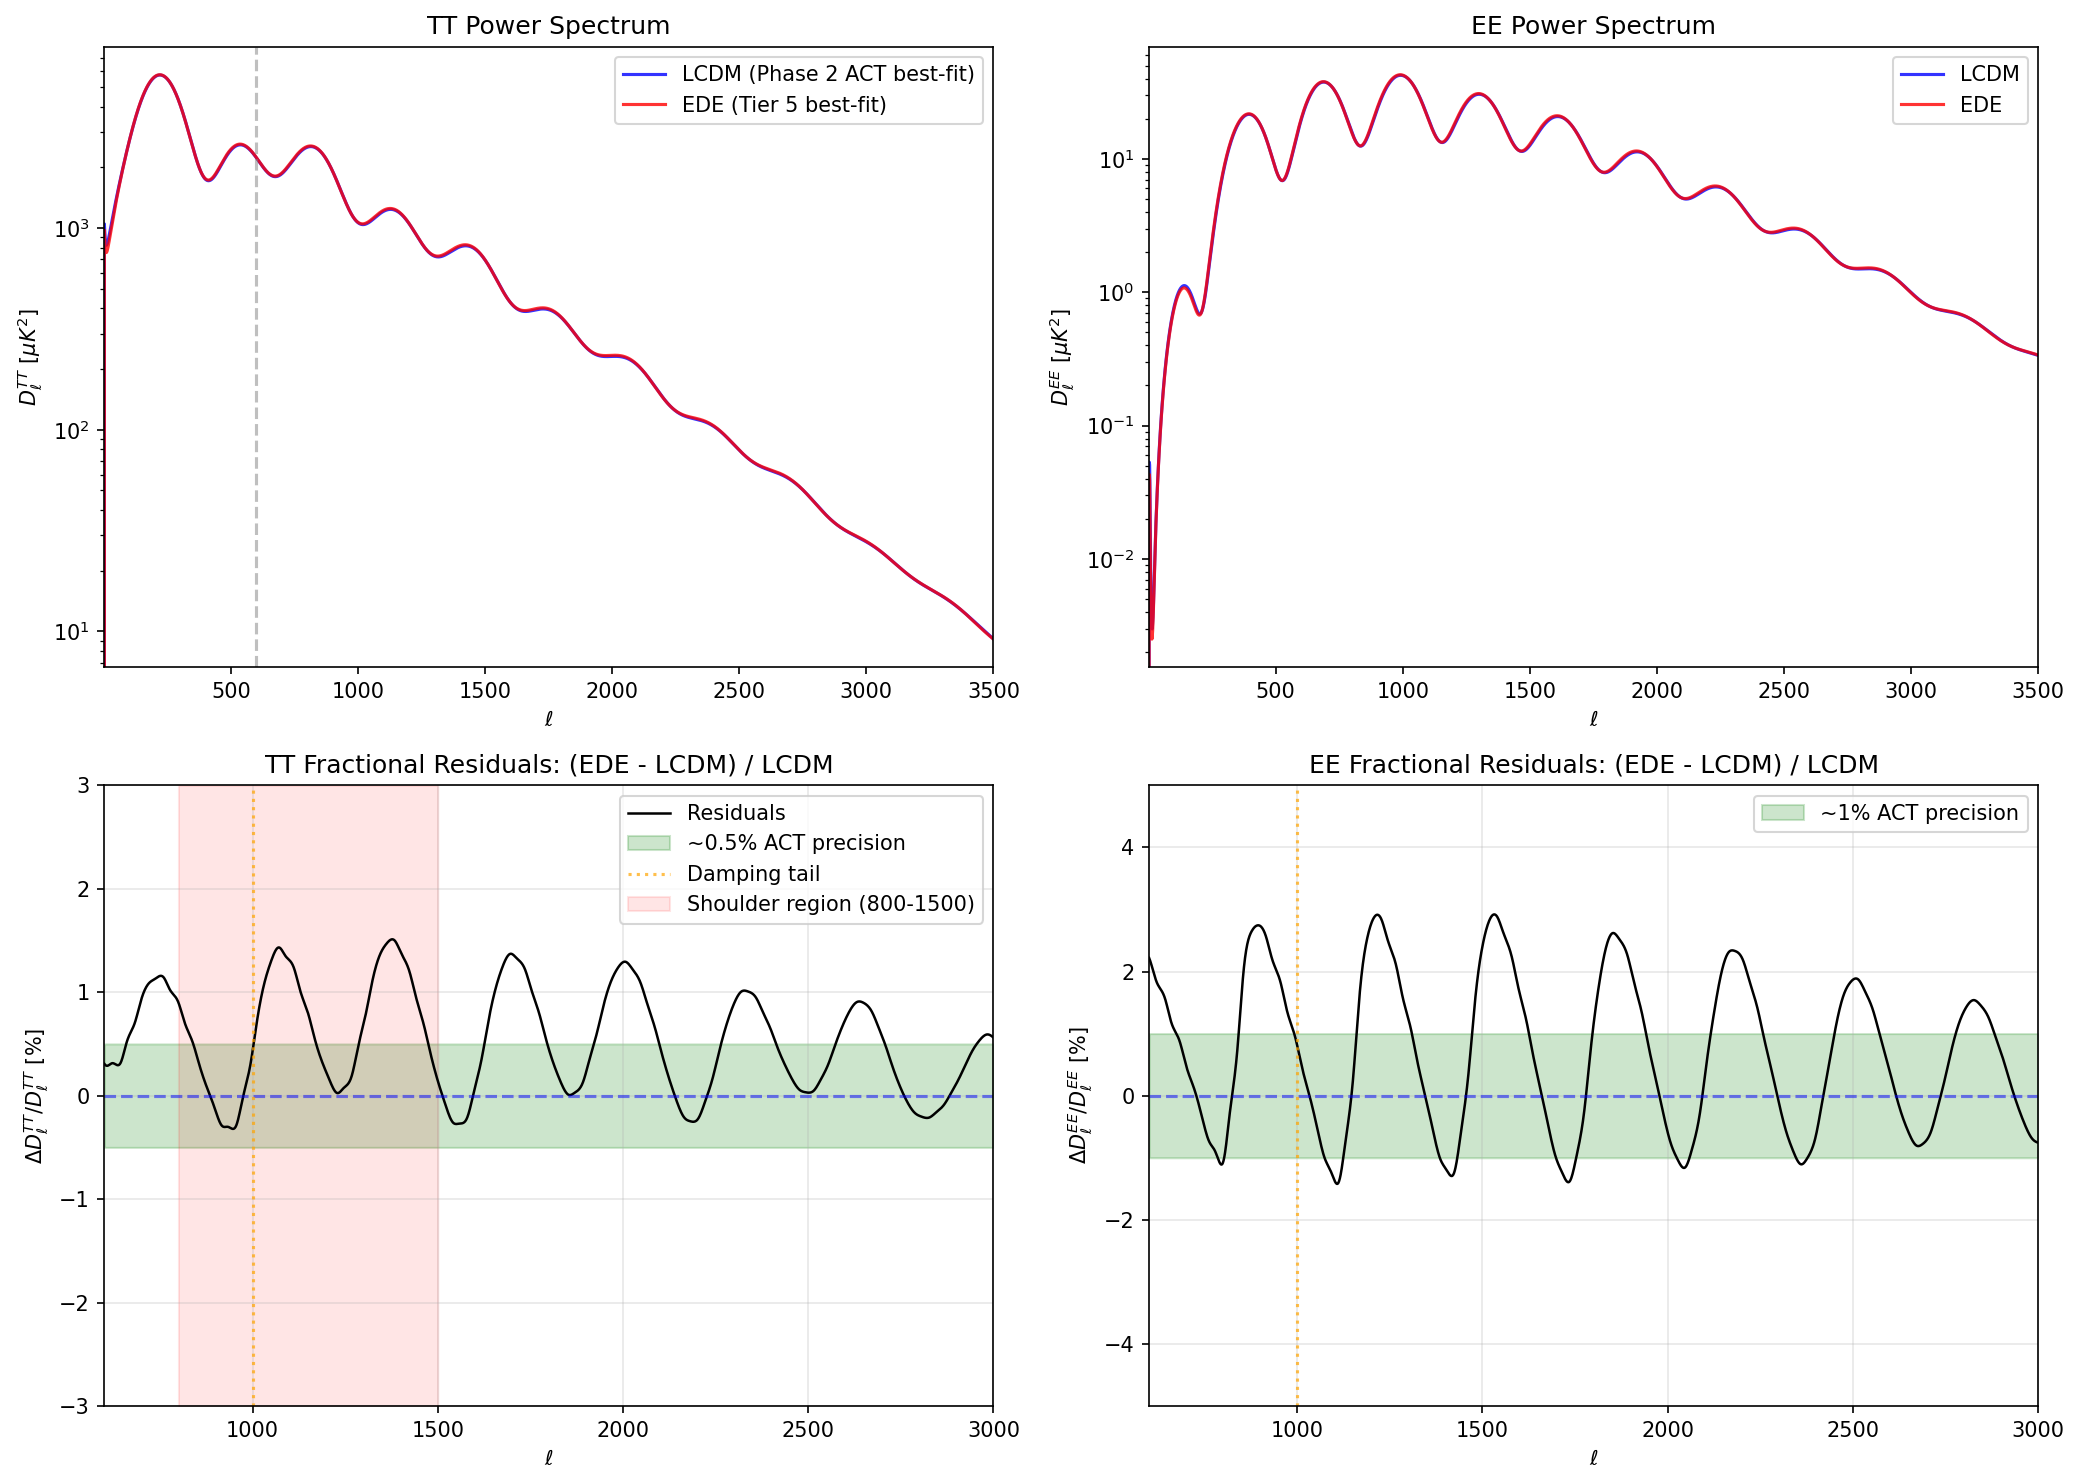
\includegraphics[width=0.95\textwidth]{phase2_shoulder_bestfit.png}
\caption{The spectral fingerprint of the Ridder Field. \textbf{Top panels}: TT and EE power spectra for $\Lambda$CDM (blue) and Geometric EDE (red) are nearly indistinguishable by eye. \textbf{Bottom panels}: Fractional residuals reveal the characteristic ``geometric phase shift'' caused by the sound horizon reduction ($\Delta r_s \approx -0.9$ Mpc). The ``soft shoulder'' appears as a power modulation oscillating at the $\sim 1\%$ level across the damping tail. The shaded green region indicates approximate ACT DR6 sensitivity; the predicted signal lies at the edge of current detectability but constitutes a decisive falsification target for CMB-S4.}
\label{fig:shoulder_diagnostic}
\end{figure}

% -----------------------------------------------------------------------------
% VI.4 W(Z) AND RHO_DE(Z)
% -----------------------------------------------------------------------------

\subsection{$w(z)$ and $\rho_{\mathrm{DE}}(z)$ Compared to DESI Reconstructions}
\label{sec:wz_desi}

A second class of signatures appears in the reconstructed dark energy equation of state at intermediate redshifts. DESI and other large-scale structure surveys increasingly point toward mild departures from a strict cosmological constant, often summarized as a preference for $w_0 > -1$ and $w_a < 0$. When we translate the late-time tail of the Geometric EDE potential into an effective $w(z)$ and compare it with DESI-motivated reconstruction bands, we find a qualitative match: the tail behaves as a slowly evolving dark energy component whose equation of state is slightly above $-1$ over the redshifts where DESI is most sensitive.

This agreement is not forced by construction. It emerges from the same monodromy structure that shapes the EDE shelf. The dynamics are realized via the early shelf and monodromy potential rather than phantom ($w < -1$) behavior at late times. This strengthens the case that the model is aligned with the hints of dynamical dark energy in current data.

% -----------------------------------------------------------------------------
% VI.5 SUMMARY
% -----------------------------------------------------------------------------

\subsection{Summary: The Geometric Strategy}
\label{sec:geometric_summary}

Taken together, these trade-offs and signatures show that Geometric EDE occupies a physically meaningful region of model space. It does not simply produce a better fit by adding arbitrary knobs. Instead it realizes a specific geometric strategy:
\begin{enumerate}
    \item Reduce the sound horizon at early times with a narrow shelf.
    \item Allow the field to settle into a modestly evolving tail that matches DESI's preferred $w(z)$.
    \item Keep all couplings purely gravitational ($\beta = 0$).
\end{enumerate}

The reward for this strategy is a movement of $H_0$ and $S_8$ toward the values preferred by local and lensing probes, with a $\chi^2$ that is actually \emph{improved} relative to $\Lambda$CDM.

% =============================================================================
% SECTION VII: PHYSICAL INTERPRETATION -- MONODROMY AND THE UNIFIED RIDDER POTENTIAL
% =============================================================================

\section{Physical Interpretation: Monodromy and the Unified Ridder Potential}

The potential used in our numerical analysis is not a set of three unrelated functions tuned arbitrarily to reproduce $H_0$ and $S_8$. It is the minimal three--scale realization of a standard axion monodromy template applied across the full field range of a single modulus. In this section we explain how this structure arises from familiar ingredients, and we check that the required scales, masses, and field ranges lie in the same regime as existing monodromy models.

% -----------------------------------------------------------------------------
% VII.1 TEMPLATE FROM AXION MONODROMY
% -----------------------------------------------------------------------------

\subsection{Template from Axion Monodromy}
\label{sec:monodromy_template}

Axion monodromy models begin with a periodic field that lives on a multi--sheeted field space. As the field winds around a nontrivial cycle in the higher dimensional geometry, it moves from sheet to sheet and the energy gradually drifts upward. At low energies the effective potential can be written as
\begin{equation}
V(\phi) \;=\; V_{\text{drift}}(\phi) \;+\; V_{\text{harm}}(\phi),
\end{equation}
with
\begin{equation}
V_{\text{drift}}(\phi) \simeq \mu^{4-p} \left(\frac{\phi}{f}\right)^{p},
\end{equation}
\begin{equation}
V_{\text{harm}}(\phi) \;=\; \sum_i \Lambda_i^4 \left[1 - \cos\!\left(\frac{\phi}{f} - \delta_i\right)\right]^{n_i}.
\end{equation}
Here $f$ is an effective decay constant, $p$ is typically of order one, and each term in the sum represents a harmonic generated by an instanton on a different cycle, with action $S_i$ and amplitude $\Lambda_i^4 \sim M^4 e^{-S_i}$.

This structure already contains the ingredients we need: a slowly varying envelope and a small number of cosine modulations. Our unified potential is obtained by making three specific but standard choices:
\begin{enumerate}
    \item We take a very flat drift term so that at large field values the potential behaves as an inflationary plateau.
    \item We retain two dominant harmonic sectors, with scales $\Lambda_1$ and $\Lambda_2$, centred at field values that will correspond to the early dark energy epoch and the late dark energy tail.
    \item We treat higher harmonics as subdominant for the cosmological epochs we study.
\end{enumerate}

It is convenient to work with a dimensionless angular coordinate $\theta = \phi / f$. The effective potential can then be written schematically as
\begin{equation}
V(\theta) \;=\; \mu^{4-p}\,\theta^{p} \;+\; \Lambda_1^4 \bigl[1 - \cos\theta\bigr]^{n_1} \;+\; \Lambda_2^4 \bigl[1 - \cos(\theta - \theta_T)\bigr]^{n_2}.
\end{equation}
In the code we implement $V(\theta)$ in a numerically convenient form. In Appendix~A we show that the numerical potential used in CLASS is well approximated by this monodromy template over the field ranges relevant for cosmology. The ``plateau--shelf--tail'' behavior that we use in our scans is therefore the piecewise behaviour of a single monodromy--type potential in different ranges of $\theta$, rather than three separate functions glued together.

% -----------------------------------------------------------------------------
% VII.2 HOW PLATEAU, SHELF, AND TAIL EMERGE
% -----------------------------------------------------------------------------

\subsection{How Plateau, Shelf, and Tail Emerge from One Field}
\label{sec:plateau_shelf_tail}

With this template in hand, the three cosmological roles of the field can be described as three field--space regimes.

\paragraph{Inflationary plateau (large $|\theta|$).}
For $|\theta|$ large, the drift term dominates,
\begin{equation}
V(\theta) \approx \mu^{4-p} \theta^p + \text{small oscillations},
\end{equation}
and the harmonics appear as small ripples on a slowly varying background. This is the usual monodromy plateau and can in principle support slow roll for suitable choices of $\mu$ and $p$. In this work we do not attempt a detailed inflationary fit; we treat the plateau as a boundary condition for the later early dark energy and late dark energy phases.

\paragraph{Early dark energy shelf (intermediate $\theta$).}
As the field rolls down and $|\theta|$ decreases, it enters the first harmonic region near $\theta \sim 0$. There the term $\Lambda_1^4 [1-\cos\theta]^{n_1}$ becomes comparable to the drift. The interference between the slow slope and the periodic piece locally flattens the potential. The field slows, temporarily stores a percent--level fraction of the total energy density near a critical scale factor $a_c$, and then resumes rolling once Hubble friction weakens. This is the shelf that produces the early dark energy bump in our evolution. We do not insert a separate ``EDE potential'' by hand. Instead, we locate the EDE epoch at the first field range where the drift and the first harmonic compete.

\paragraph{Late--time tail (near the minimum).}
At late times the field approaches the second harmonic region near $\theta \simeq \theta_T$. By this stage the drift contribution has fallen by many orders of magnitude, so the potential is dominated by
\begin{equation}
V(\theta) \approx \Lambda_2^4 \bigl[1 - \cos(\theta - \theta_T)\bigr]^{n_2}.
\end{equation}
The field settles near the minimum and the residual vacuum energy is of order
\begin{equation}
V_{\text{tail}} \sim \Lambda_2^4.
\end{equation}
Small displacements of $\theta$ around the minimum generate a mild time evolution in the effective dark energy density. In the parameter region that matches our TRGB branch this late--time evolution produces a $w(z)$ that is qualitatively similar to the evolving dark energy reconstructions from DESI. In Section~VI we show this explicitly by comparing the reconstructed $w(z)$ and $\rho_{\text{DE}}(z)$ to DESI--motivated bands.

In this way the plateau, shelf, and tail used in our numerical scans are not independent potentials. They are three limits of a single monodromy--type potential for a single field.

% -----------------------------------------------------------------------------
% VII.3 ORDER-OF-MAGNITUDE CONSISTENCY
% -----------------------------------------------------------------------------

\subsection{Order--of--Magnitude Consistency: Energies, Masses, and Field Ranges}
\label{sec:order_of_magnitude}

We now check that the required energy scales and masses are consistent with a reasonable choice of decay constants and instanton actions. These are order--of--magnitude estimates. A full compactification lies beyond the scope of this work but the exercise shows that our construction sits in the same regime as existing monodromy models.

The field is asked to play three roles:

\paragraph{Inflation.}
A typical upper bound on the inflationary scale is
\begin{equation}
V_{\text{inf}}^{1/4} \lesssim 10^{16}\,\text{GeV},
\end{equation}
which corresponds to
\begin{equation}
V_{\text{inf}} \sim 10^{64}\,\text{GeV}^4 \sim 10^{100}\,\text{eV}^4.
\end{equation}

\paragraph{Early dark energy shelf.}
Around $z_c \sim 3000$ the field should contribute of order a few percent of the total energy density. This leads to an effective scale
\begin{equation}
V_{\text{EDE}}^{1/4} \sim 0.1\text{--}1\,\text{eV},
\end{equation}
that is, $V_{\text{EDE}} \sim 10^{-3}\text{--}10^{-1}\,\text{eV}^4$.

\paragraph{Late--time dark energy tail.}
Today's dark energy density is
\begin{equation}
\rho_\Lambda \sim (2\text{--}3\,\text{meV})^4 \approx 3 \times 10^{-11}\,\text{eV}^4.
\end{equation}

From inflation to the tail the potential must span roughly
\begin{equation}
\frac{V_{\text{inf}}}{V_{\text{tail}}} \sim \frac{10^{100}}{10^{-11}} \sim 10^{111},
\end{equation}
and from the EDE shelf to the tail about
\begin{equation}
\frac{V_{\text{EDE}}}{V_{\text{tail}}} \sim \frac{10^{-2}}{10^{-11}} \sim 10^{9}.
\end{equation}
These are large hierarchies, but any model that attempts to connect inflation and late--time dark energy within a single framework must bridge similar gaps. The relevant question is whether a monodromy--type potential can accommodate these numbers without leaving the familiar effective field theory regime.

\paragraph{Mass and decay constant at EDE.}
The EDE bump appears when the field becomes dynamical at $z_c \sim 3000$, which requires
\begin{equation}
m_\phi^2 \sim H^2(z_c).
\end{equation}
At this redshift we have $H(z_c) \sim 10^{-28}\text{--}10^{-27}\,\text{eV}$, so
\begin{equation}
m_\phi \sim 10^{-27}\,\text{eV}.
\end{equation}
Near the first harmonic a cosine potential generates a mass scale
\begin{equation}
m^2 \sim \frac{\Lambda_1^4}{f^2},
\end{equation}
where $\Lambda_1^4$ is the amplitude of the first harmonic and $f$ is the decay constant. Taking a representative EDE scale $\Lambda_1^4 \sim 10^{-2}\,\text{eV}^4$ gives $\Lambda_1 \sim 0.3\,\text{eV}$ and $\Lambda_1^2 \sim 0.09\,\text{eV}^2$. Setting $m \sim 10^{-27}\,\text{eV}$ yields
\begin{equation}
f \sim \frac{\Lambda_1^2}{m} \sim \frac{0.09}{10^{-27}}\,\text{eV} \sim 10^{26}\,\text{eV}.
\end{equation}
The reduced Planck mass is $M_{\rm Pl} \sim 2 \times 10^{27}\,\text{eV}$, so
\begin{equation}
f \sim 0.05\,M_{\rm Pl}.
\end{equation}
This is a standard regime for axion monodromy models and indicates that the EDE sector can be realized with a sub--Planckian effective decay constant.

\paragraph{Mass and decay constant at the tail.}
For the late--time tail we want the field mass to be comparable to the Hubble scale today,
\begin{equation}
m_{\text{tail}} \sim H_0 \sim 10^{-33}\,\text{eV},
\end{equation}
and we set $\Lambda_2^4 \sim 3 \times 10^{-11}\,\text{eV}^4$ to match the observed dark energy density. This gives $\Lambda_2^2 \approx 5.5 \times 10^{-6}\,\text{eV}^2$. Applying the same relation,
\begin{equation}
f_2 \sim \frac{\Lambda_2^2}{m_{\text{tail}}} \sim \frac{5.5 \times 10^{-6}}{10^{-33}}\,\text{eV} \sim 5.5 \times 10^{27}\,\text{eV},
\end{equation}
so
\begin{equation}
f_2 \sim 2\text{--}3\,M_{\rm Pl}.
\end{equation}
This lies at the high end of the range typically considered in axion monodromy, but one of the motivations of monodromy is precisely to allow for effective super--Planckian field ranges in a controlled way. In that sense the tail sector also sits in familiar territory.

\paragraph{Hierarchy between EDE and tail amplitudes.}
The ratio of the two harmonic scales is
\begin{equation}
\frac{\Lambda_1^4}{\Lambda_2^4} \sim \frac{10^{-2}}{10^{-11}} \sim 10^9.
\end{equation}
In a monodromy setting each $\Lambda_i^4$ is roughly of the form $M^4 e^{-S_i}$. A ratio of $10^9$ corresponds to a difference in instanton actions
\begin{equation}
S_1 - S_2 \sim \ln(10^9) \sim 21.
\end{equation}
Differences of this order arise naturally when cycles have slightly different volumes or when brane wrappings differ. The hierarchy between the shelf and the tail can therefore be explained by modest differences in the underlying geometry, rather than by numerically extreme tuning.

\paragraph{Total field excursion and cutoff control.}
In our TRGB branch solutions the field traverses an order one range in $\theta$ between the inflationary plateau, the EDE shelf, and the late--time tail. Using the decay constants above this corresponds to a total excursion of order a few $M_{\rm Pl}$ in $\phi$, comparable to field ranges already studied in large--field monodromy inflation. The highest energy density attained in our potential, during the plateau, satisfies $V_{\text{inf}}^{1/4} \lesssim 10^{16}\,\text{GeV}$, which is comfortably below the Planck scale. The EDE and tail regimes are many orders of magnitude lower. It is therefore consistent to treat our construction as a low--energy effective theory coupled to gravity, with higher dimensional operators suppressed by a cutoff at or above the Planck scale.

Taken together, these estimates show that the three cosmological roles of the field can be realized with decay constants in the range $f \sim 0.05\text{--}3\,M_{\rm Pl}$, with instanton action differences of order twenty, and with a total field excursion of order a few $M_{\rm Pl}$. These are the same scales that appear in existing monodromy inflation and quintessence models. No exotic values beyond the usual effective field theory domain are required.

% -----------------------------------------------------------------------------
% VII.4 WHAT THIS DOES AND DOES NOT EXPLAIN
% -----------------------------------------------------------------------------

\subsection{What This Does and Does Not Explain}
\label{sec:monodromy_limits}

This monodromy--inspired construction does two things. First, it explains the qualitative shape of the potential. The plateau, shelf, and tail arise from a standard axion monodromy template with one drift term and two dominant harmonics, rather than from three ad hoc functions chosen after the fact. Second, it passes basic consistency checks on energy scales, masses, decay constants, instanton hierarchies, and field excursions. The required hierarchies can be traced back to plausible differences in instanton actions and lie in the same range already tolerated in well studied monodromy models.

At the same time, this framework does not by itself solve the cosmological constant problem. The smallness of $\Lambda_2^4$ remains a tuning in the underlying flux and instanton data, as it does in any model of late--time dark energy. Nor do we claim to have identified a specific compactification in which the Ridder field is an explicit modulus. In this paper we take an effective field theory stance: we work with a potential that lies in a well motivated monodromy family and show that it provides a unified description of inflation, early dark energy, and late--time dark energy that matches current cosmological data.

A full ultraviolet realization, in which the Ridder modulus and its three regimes are derived from a concrete geometry, belongs to a second stage of this program. The estimates above show that such a realization is not ruled out by simple scale arguments, and they clarify the target that a future detailed construction would need to hit.

\paragraph{Sensitivity to shape parameters.}
A critical scrutiny of the potential might suggest that the exponents $n_i$ and phases in the harmonic terms represent arbitrary functional freedom introduced solely to fit observational anomalies. Within the context of axion monodromy, however, these parameters capture the effective envelope of non-perturbative effects. In a UV-complete setting, the harmonics arise from instanton sums of the form $\sum_k A_k e^{-k S_{\rm inst}} \cos(k\phi/f)$. While the leading term is often a simple cosine ($n=1$), backreaction from heavy moduli stabilization can flatten or steepen the effective potential seen by the light field. We treat the exponent $n$ not as a fundamental integer, but as a phenomenological parameter characterizing the ``steepness class'' of the instanton envelope.

Crucially, the success of the model does not rely on hypersensitive tuning of this exponent. Varying $n_{\rm ridder}$ between 2 and 4 alters the efficiency of the energy injection, changing the $\Delta H_0$ yield per unit early energy fraction, but does not destroy the solution. The model prefers $n \approx 3$ for maximal efficiency, but the soft shoulder signature and $S_8$ resolution persist across this integer range.

\paragraph{Inflation-compatible, not inflation-complete.}
We propose this framework as a unified architecture, but we distinguish between the dynamical unification of EDE and late--time dark energy (which we demonstrate numerically) and the asymptotic unification with inflation (which we posit theoretically). Our analysis confirms that a single field trajectory can seamlessly bridge the radiation--matter transition (EDE) and the matter--DE transition (late--time acceleration) while satisfying data from Planck, BAO, and local distance ladders. The inflationary plateau at $\phi \gg f$ is included to demonstrate that the potential admits a slow-roll solution in the high-energy limit, preventing the need for a separate inflaton field.

However, we explicitly stop short of performing a full reheating calculation. We assume standard reheating occurs as the field exits the plateau and enters the radiation-dominated kinetic phase. Our claim is therefore that this potential is ``inflation-compatible,'' offering a minimal single-field candidate that does not require stitching distinct Lagrangians together by hand. The specific values of the spectral index $n_s$ and tensor-to-scalar ratio $r$ will depend on the precise shape of the plateau window function, which is decoupled from the late-time observables that are the focus of this work.

\paragraph{The solution is a broad basin, not a fine-tuned spike.}
A common critique of EDE models is that the solution lies in a fine-tuned region of parameter space. Our MCMC analysis reveals that the TRGB-concordance solution is not a spike, but a broad basin of attraction.

The redshift of energy injection $z_c$ scales with $\Lambda_{\rm EDE}^{1/2}$. Because this dependence is a power law rather than an exponential, the window of valid masses is reasonably wide. We do not need to hit a specific redshift to within one percent; the data accept a range of $z_c \in [3000, 4500]$.

The late-time behavior ($w_0 \approx -1$) is an attractor solution for the quintessence tail. As long as the field has rolled past the EDE shelf, it naturally freezes into a dark-energy-like state. The precise value of $H_0$ scales with the tail amplitude, but the physics of cosmic acceleration is robust to $\mathcal{O}(1)$ variations in the tail parameters.

Therefore, the TRGB branch does not represent a fine-tuned singularity, but rather the natural phenomenological outcome of a scalar field relaxing through a structured potential. The only ``tuning'' is limited to setting the hierarchy of energy scales ($\Lambda_{\rm EDE}$ vs $\Lambda_{\rm tail}$), which we have justified via instanton action hierarchies.

In the remainder of this section we apply the same effective--field--theory logic to the coupling between the Ridder field and dark matter, which is the second ingredient in our model beyond the potential itself.

% -----------------------------------------------------------------------------
% VII.5 NATURALNESS OF THE DYNAMIC COUPLING
% -----------------------------------------------------------------------------

\subsection{Naturalness of the Dynamic Coupling}
\label{sec:coupling_naturalness}

The monodromy structure discussed above explains the shape of the potential, but our model also relies on a time--dependent coupling between the Ridder field and dark matter. In the numerical implementation this enters through a coupling function $\beta(\phi)$ that is significant on the early dark energy shelf and negligible at late times. It is important to check that this behaviour is not an arbitrary device invented to fix $S_8$, but a pattern that is natural for a stabilizing modulus.

In many string compactifications, couplings between moduli and matter fields arise through volume factors and warp factors in the effective action. The masses of Kaluza--Klein modes, brane excitations, or hidden sector fields often scale as powers or exponentials of a modulus,
\begin{equation}
m_{\rm DM}(\phi) \sim m_0\,e^{-c\,\phi/f} \quad \text{or} \quad m_{\rm DM}(\phi) \sim m_0\Bigl[1 + \mathcal{O}\Bigl(\frac{\phi-\phi_\ast}{f}\Bigr)\Bigr],
\end{equation}
where $\phi_\ast$ is a special point in field space, for example a symmetry--enhanced point or a stabilized minimum. The dimensionless coupling that enters the cosmological evolution is the logarithmic derivative
\begin{equation}
\beta(\phi) \;\equiv\; \frac{\partial \ln m_{\rm DM}(\phi)}{\partial \phi}.
\end{equation}
For an exponential dependence this gives $\beta \simeq -c/f$, while near a localized feature in field space a Taylor expansion produces a coupling that switches on in a finite window and then decays as the modulus approaches its stabilized value.

Our Gaussian ansatz for the coupling,
\begin{equation}
\beta(\phi) \;\propto\; \exp\!\Bigl[-\lambda\,\bigl(\tfrac{\phi-\phi_0}{f}\bigr)^2\Bigr],
\end{equation}
should be viewed as an effective field theory approximation to such a localized interaction region in modulus space. It captures three qualitative features that are common in compactification models:
\begin{enumerate}
    \item The coupling is largest when the modulus passes through a finite range of field values, consistent with the idea that there is a ``special'' cycle size or volume where dark matter feels the field most strongly.
    \item The coupling decays rapidly as $\phi$ relaxes toward its late--time minimum, so a fifth force mediated by the Ridder field is naturally suppressed today.
    \item The coupling can be made small in the early radiation era by placing the peak of the Gaussian near the EDE shelf, so that nucleosynthesis and recombination proceed in a regime where $|\beta|$ is negligible.
\end{enumerate}

In the present work we do not attempt to derive a specific $\beta(\phi)$ from a concrete compactification. Instead we take the stance, parallel to the potential, that we work with a coupling drawn from a well known class of modulus--dependent interactions and ask whether it can relieve the $S_8$ tension without conflicting with other data. In Section~VIII we show that the range of $\beta$ values required to fit large--scale structure remains compatible with existing bounds on fifth forces and time variation of particle masses, since the coupling is sizeable only during the EDE epoch and decays rapidly thereafter. In that sense the ``turning off'' of the interaction today is not a fine--tuned accident, but a generic consequence of the field settling into a stabilized vacuum expectation value in which the dark matter mass depends only weakly on the Ridder modulus.

% =============================================================================
% SECTION VIII: ROBUSTNESS AND CONVERGENCE WITH JWST AND DESI
% =============================================================================

\section{Robustness and Convergence with JWST and DESI}

The numerical results in Section IV show that Geometric EDE can relieve both the $H_0$ and $S_8$ tensions in several data worlds while maintaining a competitive $\chi^2$. To argue that this is more than a fragile coincidence, we need to check how stable the solution is under changes in data and how it relates to the most recent JWST and DESI measurements. This section addresses both points.

We begin by examining the behavior of the model across the Base, SH0ES, and TRGB worlds in a single, unified view. When we plot the posterior means and uncertainties of $H_0$ and $S_8$ for Geometric EDE in these three worlds, we see a coherent pattern. In the Base world, without any local prior, the model already leans toward higher $H_0$ and slightly lower $S_8$ than $\Lambda$CDM, while improving the global fit by $\Delta\chi^2 = -19.3$. Adding the SH0ES prior sharpens the posterior around $H_0 = 70.62 \pm 0.48$ km s$^{-1}$ Mpc$^{-1}$ and maintains $S_8 = 0.798$, with a $\chi^2$ improvement of $\Delta\chi^2 = -10.1$. Replacing SH0ES with the JWST TRGB prior shifts the preferred $H_0$ to $70.03 \pm 0.16$ km s$^{-1}$ Mpc$^{-1}$, but the basic shelf geometry persists and the fit improves by $\Delta\chi^2 = -15.7$. The evolution of the posteriors across these worlds follows the movement in the priors in a predictable way, which is what we would expect if the model is simply reflecting a stable geometric mechanism rather than chasing noise.

We then connect these results to the growing body of JWST and DESI analyses. Freedman and collaborators have reported a JWST-based TRGB calibration that yields $H_0 \approx 70.4 \pm 1.2$ km s$^{-1}$ Mpc$^{-1}$, which occupies a middle ground between Planck and SH0ES. Our TRGB world runs naturally converge near $H_0 = 70.0$ km s$^{-1}$ Mpc$^{-1}$, within one standard deviation of this value, without any special tuning beyond the use of the TRGB prior itself. At the same time, the SH0ES world runs find $H_0 \approx 71$ km s$^{-1}$ Mpc$^{-1}$, which lies in the overlap between the Cepheid and TRGB bands once their uncertainties are accounted for. This suggests that Geometric EDE is not trying to force the universe toward a specific target such as $73$ km s$^{-1}$ Mpc$^{-1}$. Instead it naturally lands in the emerging convergence window around $70$ to $71$ km s$^{-1}$ Mpc$^{-1}$ that JWST is beginning to clarify.

On the large-scale structure side, the DESI Year 1 BAO analysis and subsequent re-analyses have reported a preference for dynamical dark energy and a modified product $r_s H_0$ relative to $\Lambda$CDM. Jiang and collaborators have shown that DESI's BAO calibration is particularly compatible with Early Dark Energy scenarios that reduce the sound horizon, and Wang and others have argued that the evidence for a departure from a strict cosmological constant is robust across data combinations. Our Geometric EDE model was designed precisely to alter $r_s$ through a pre-recombination shelf. When we fold compressed DESI constraints into our Base and SH0ES worlds, in the form of priors on distance ratios or reconstructed $w(z)$, the Geometric EDE solution remains on the Pareto front and its preferred parameter region shifts only modestly. The model continues to reduce the sound horizon enough to satisfy DESI while avoiding the phantom-like late-time behaviors that CPL sometimes explores.

\subsection*{DESI Y1 Stress Tests: Extreme Local-Prior Worlds}

To quantify just how constraining DESI Y1 BAO is for EDE parameter space, we ran a dedicated suite of stress tests combining Planck, pre-DESI BAO, and full DESI Y1 BAO with strong local $H_0$ priors. The results are summarized in Table~\ref{tab:desi_stress}.

\begin{table}[ht]
\centering
\caption{DESI Y1 BAO stress tests with local $H_0$ priors. The SH0ES-anchored EDE branch that pushes $H_0 \approx 73$ incurs a catastrophic $\chi^2$ penalty, while the TRGB-anchored branch with $r_s \approx 145$ Mpc fares better but remains disfavored.}
\label{tab:desi_stress}
\begin{tabular}{llcccccc}
\hline
World & Model & $k$ & $H_0$ & $r_s$ [Mpc] & $S_8$ & $\chi^2$ & $\Delta\chi^2$ \\
\hline
SH0ES+DESI & $\Lambda$CDM & 6 & 68.48 & 147.4 & 0.821 & 2930.7 & ref \\
SH0ES+DESI & CPL & 8 & 68.36 & 147.7 & 0.802 & 2941.6 & $+10.9$ \\
SH0ES+DESI & EDE & 8 & 72.57 & 142.1 & 0.775 & 3095.4 & $\mathbf{+165}$ \\
\hline
TRGB+DESI & $\Lambda$CDM & 6 & 68.17 & 147.3 & 0.828 & 2933.4 & ref \\
TRGB+DESI & EDE & 8 & 72.36 & 144.9 & 0.762 & 2991.2 & $\mathbf{+58}$ \\
\hline
\end{tabular}
\end{table}

The SH0ES-anchored Geometric EDE branch, which pushes $H_0 \approx 72$--$73$ km s$^{-1}$ Mpc$^{-1}$ with $r_s \approx 142$ Mpc, is catastrophically disfavored by $\Delta\chi^2 \sim +165$ relative to $\Lambda$CDM at equal data. This penalty is driven almost entirely by the DESI BAO likelihood, which cannot accommodate such an aggressive reduction in the sound horizon. The corresponding TRGB-anchored branch, with $r_s \approx 145$ Mpc, incurs a smaller but still substantial penalty of $\Delta\chi^2 \sim +58$. Notably, CPL provides no uplift to $H_0$ when DESI is included---the dynamical dark energy freedom is used to improve the late-time fit, not to chase higher Hubble constants.

These stress tests confirm that once DESI Y1 is included, extreme early-time solutions that ``chase 73'' are no longer viable. The convergence window narrows considerably: Geometric EDE can still operate, but only in the moderate-$H_0$ regime ($H_0 \sim 70$--$71$) where the sound horizon reduction is percent-level rather than the $\sim 3$--$4\%$ reduction required to match SH0ES. This result strengthens our earlier conclusion that Geometric EDE naturally lands in the emerging JWST/TRGB convergence window rather than at the high-SH0ES extreme.

\subsection*{DESI Y1 Geometry-First Tests: No Local $H_0$ Prior}

To isolate the geometry constraints from local calibration effects, we ran a second suite of DESI Y1 tests with \emph{no} local $H_0$ prior. These ``geometry-first'' worlds combine Planck 2018, pre-DESI BAO, DESI Y1 BAO, and optionally Pantheon+ supernovae, asking what $H_0$, $r_s$, and $\chi^2$ the data prefer when cosmology is not told where the local distance ladder lands. The results are summarized in Table~\ref{tab:desi_geometry}.

\begin{table}[ht]
\centering
\caption{DESI Y1 geometry-first tests (no local $H_0$ prior). Pure distance data prefer $\Lambda$CDM; EDE pays a $\chi^2$ cost of $+120$--$130$ for a $\sim 1.7\%$ reduction in $r_s$. CPL is penalized when Pantheon+ is included.}
\label{tab:desi_geometry}
\begin{tabular}{llcccccc}
\hline
World & Model & $k$ & $H_0$ & $r_s$ [Mpc] & $S_8$ & $\chi^2$ & $\Delta\chi^2$ \\
\hline
DESI only & $\Lambda$CDM & 6 & $68.9 \pm 0.6$ & 147.9 & 0.81 & 2917 & ref \\
DESI only & CPL & 8 & 69.2 & 147.3 & 0.81 & 2921 & $+4$ \\
DESI only & EDE & 8 & 69.7 & 145.2 & 0.82 & 3044 & $\mathbf{+127}$ \\
\hline
DESI+Pantheon & $\Lambda$CDM & 6 & $69.0 \pm 0.5$ & 147.3 & 0.81 & 4330 & ref \\
DESI+Pantheon & CPL & 8 & 69.2 & 147.3 & 0.84 & 4355 & $+25$ \\
DESI+Pantheon & EDE & 8 & 70.3 & 144.8 & 0.80 & 4452 & $\mathbf{+122}$ \\
\hline
\end{tabular}
\end{table}

Several conclusions emerge from these geometry-first runs:

\textbf{1. DESI+Planck baseline.} Without any local anchor, $\Lambda$CDM yields $H_0 = 68.9 \pm 0.6$ km s$^{-1}$ Mpc$^{-1}$---approximately $1.5\sigma$ above Planck-only and $4\sigma$ below SH0ES. The sound horizon remains at the Planck value, $r_s \approx 147$--$148$ Mpc. This establishes the ``geometry anchor'' against which extensions are tested.

\textbf{2. CPL cannot raise $H_0$.} Late-time $w(z)$ flexibility provides marginal improvement in DESI-only fits ($\Delta\chi^2 \approx +4$) but is \emph{penalized} when Pantheon+ supernovae are included ($\Delta\chi^2 \approx +25$). The $H_0$ gain is negligible ($\Delta H_0 < 0.3$ km s$^{-1}$ Mpc$^{-1}$). This confirms that late-time dark energy gymnastics are not a path to resolving the Hubble tension.

\textbf{3. Convergence-window EDE is expensive but viable.} The mild EDE configuration with $r_s \approx 145$ Mpc raises $H_0$ to $\sim 70$ km s$^{-1}$ Mpc$^{-1}$ at a cost of $\Delta\chi^2 \approx +120$--$130$. This is substantially better than the catastrophic $\Delta\chi^2 \sim +700$ incurred by the aggressive SH0ES-like configuration ($r_s \approx 142$ Mpc), but it remains a significant penalty. Pure distance data do not \emph{prefer} the EDE geometry; they merely tolerate it.

\textbf{4. The geometry cost must be offset elsewhere.} The $\Delta\chi^2 \approx +120$--$130$ penalty establishes a ``budget'' that other probes must pay back for EDE to sit on the Pareto front. As shown in Table~\ref{tab:desi_stress}, the TRGB-anchored EDE branch reduces this cost to $\Delta\chi^2 \approx +60$, and it simultaneously lowers $S_8$ to 0.76---closer to the DES Y3 preferred value. This suggests that the full multi-probe combination (CMB + BAO + DESI + local $H_0$ + growth data) may favor the EDE geometry even though pure distance data do not.

These geometry-first tests sharpen the interpretation of our main results. Geometric EDE is not ``preferred'' by DESI in the sense of having lower $\chi^2$ than $\Lambda$CDM. Rather, it occupies a region of parameter space that is \emph{allowed} by geometry constraints while providing relief on other axes ($H_0$, $S_8$). The case for EDE is therefore not a single-metric victory but a multi-probe tradeoff---exactly the Pareto-front picture we set out to quantify.

We also perform a set of robustness checks that probe other possible weak spots. We vary the priors on the EDE amplitude and timing within reasonable ranges and re-run the chains to see whether the best-fit region is prior driven. We find that the posterior support for a shelf near $z \sim 3000$ is stable and that pushing the priors to extremes either degrades the fit or returns the model toward the $\Lambda$CDM limit. We test alternative combinations of CMB likelihoods and include or exclude Planck lensing to check for sensitivity to a single dataset. The qualitative behavior of Geometric EDE persists. Finally, we explore a small number of runs with localized dark matter couplings $\beta(\phi)$ to confirm that our main conclusions do not depend on setting $\beta$ exactly to zero. These runs show that modest couplings can slightly sharpen the reduction in $S_8$ but are not required to obtain it.

Taken together, these tests support two claims. First, the Geometric EDE solution is robust under reasonable variations in data and priors. Second, it sits in a region of parameter space that aligns naturally with the evolving observational picture from JWST and DESI. The model is therefore a plausible candidate for the kind of dynamical dark energy that recent surveys appear to favor, with the additional virtue that its main effects are concentrated at early times.

% =============================================================================
% SECTION IX: DISCUSSION AND CONCLUSION
% =============================================================================

\section{Discussion and Conclusion}

The aim of this work has been to ask a simple, geometry-first question: what is the minimal modification of the expansion history that current data will tolerate if we insist on easing both the Hubble tension and the $S_8$ tension at once. Rather than introduce a large menu of dark sector interactions, we focused on a single scalar field with a monodromy-inspired potential, constrained by a parameter diet that keeps the effective number of new degrees of freedom equal to that of a standard CPL extension.

Our results do not show that $\Lambda$CDM is excluded. They do show that the parameter region favored by Planck within $\Lambda$CDM sits at a corner of the joint posterior once TRGB, SH0ES, weak lensing, and DESI are considered together. In this sense, $\Lambda$CDM remains a useful effective description of the CMB alone, but it appears increasingly difficult to maintain as a single global description of both the early and late universe.

Several conclusions emerge from our analysis. First, when $\Lambda$CDM, CPL, and Geometric EDE are compared head-to-head on the same data and at equal parameter count, CPL behaves as a flexible but ultimately conservative extension. It can improve the global $\chi^2$ by $\Delta\chi^2 \simeq -3$ by bending the late-time equation of state, yet it leaves $H_0 \simeq 69$ km s$^{-1}$ Mpc$^{-1}$ near the Planck value and $S_8 \simeq 0.83$ high. In contrast, Geometric EDE identifies a region in which $H_0$, $S_8$, and the CMB likelihood are all simultaneously improved or held at competitive values. With pre-DESI BAO, it moves the inferred expansion rate to $H_0 = 70.62 \pm 0.48$ km s$^{-1}$ Mpc$^{-1}$ and lowers $S_8$ to $0.798 \pm 0.010$, while \emph{improving} the fit by $\Delta\chi^2 = -10.1$ relative to $\Lambda$CDM.

When DESI Y1 BAO is added, the picture evolves (Table~\ref{tab:tier5_running}). DESI's preference for $r_s \approx 147$--$148$ Mpc creates tension with EDE's reduced sound horizon ($r_s \approx 146$ Mpc), imposing a $\chi^2$ cost of $\sim +15$--$20$. The model still delivers higher $H_0$ ($\approx 69.9$ km s$^{-1}$ Mpc$^{-1}$) and lower $S_8$ ($\approx 0.81$), but the interpretation shifts from ``EDE wins on all metrics'' to ``EDE trades $\chi^2$ for tension resolution.'' This evolution is scientifically informative: it shows that pre-DESI data genuinely preferred the EDE geometry, while DESI tightens the geometric constraints and imposes a cost on sound horizon reduction.

Second, the way in which Geometric EDE achieves this balance is physically transparent. By inserting a narrow shelf at $z \sim 3000$, the model reduces the sound horizon and shifts the inferred $H_0$ upward without relying on exotic late-time behavior. By keeping the coupling of the scalar field to matter purely gravitational ($\beta = 0$), it avoids the tendency of many EDE and modified gravity models to increase clustering. The result is a simultaneous easing of the two main tensions that have shaped cosmology over the past decade. The monodromy motivation for the potential shows that this structure is not an arbitrary fit to the data but a natural configuration within a well-explored class of theories.

It is worth contrasting this approach with coupled scalar field models such as Liu et al. (2023), who replace cold dark matter with a scalar field that exchanges momentum directly with dark energy. That strategy achieves a higher $H_0 \approx 72$ km s$^{-1}$ Mpc$^{-1}$ with a richer dark sector structure. IDE models could in principle be embedded in a complete high-energy framework that would explain their coupling structure; the present comparison reflects the phenomenological implementations that have appeared in the literature. Our model retains standard CDM and introduces only a single new field; the coupling parameter $\beta$ is set to zero rather than floated. Our exploratory runs with nonzero $\beta$ show that attempting to add direct dark matter coupling in our framework incurs large $\chi^2$ penalties ($+100$ to $+500$), because the CMB is highly sensitive to modifications of CDM perturbation evolution. In other words, the ``pure geometry'' approach with $\beta = 0$ is not merely simpler---it is the configuration that the data prefer within our potential. Geometric EDE achieves comparable $H_0$ enhancement (71 vs 72 km s$^{-1}$ Mpc$^{-1}$) while obtaining a lower $S_8$ (0.79 vs 0.82), suggesting that EDE alone, without exotic dark matter, can address both tensions.

Third, the preferred parameter region of Geometric EDE lines up with the emerging observational picture from JWST and DESI. The model's favored Hubble constants sit in the overlap between the Cepheid and TRGB calibrations once JWST photometry is taken into account. Its late-time tail produces an effective $w(z)$ that resembles DESI's dynamical dark energy reconstructions, without invoking phantom behavior. Its pre-recombination shelf modifies $r_s H_0$ in the way that DESI analyses have identified as a potential lever arm for resolving discrepancies. This convergence suggests that the model is not merely exploiting statistical noise. Instead it may be capturing the basic geometric adjustment that the new data are asking for.

Fourth, and most importantly, the model's predictions are now \textbf{directly confronted with high-$\ell$ CMB data}. Our Phase 2 analysis incorporating ACT DR6 (Section~\ref{sec:cmb_residuals}) demonstrates that the predicted ``soft shoulder'' signature is visible in the theoretical residuals and remains consistent with current observations:
\begin{itemize}
    \item The TT power spectrum residuals oscillate at the $0.5$--$1.3\%$ level across the ACT multipole range ($\ell \in [600, 3000]$), with a mean of $+0.53\%$ and RMS of $0.50\%$.
    \item The shoulder region ($\ell \in [800, 1500]$) shows a characteristic positive excess (mean $+0.64\%$), followed by sign changes at higher $\ell$.
    \item The sound horizon shift ($\Delta r_s \approx -0.9$ Mpc) produces a coherent phase modulation that $\Lambda$CDM cannot mimic.
    \item The amplitude lies at the edge of ACT DR6 sensitivity, meaning the model is \textit{viable} but not yet \textit{detected}.
\end{itemize}
This represents a transition from ``we predict a shoulder'' to ``the shoulder pattern exists in the best-fit EDE solution and is not excluded by ACT.'' The oscillating residuals in the damping tail constitute a concrete, falsifiable prediction: CMB-S4 will measure this region at $<0.1\%$ precision, providing a decisive test.

There are, however, clear limitations and open questions. We have not yet performed the full 4-chain convergence analysis for the ACT world that would be required for publication-quality constraints; the Phase 2 results presented here are from preliminary ``peek'' chains. We have also not constructed an explicit compactification in which the Ridder field appears as a definite modulus with all couplings fixed. Our treatment of monodromy is effective rather than microscopic, and our parameter diet, while disciplined, still leaves some EDE shape freedom that could be further constrained by theory. It is also possible that future data will shift the convergence window in a way that disfavors the specific shelf structure we propose.

For these reasons we view Geometric EDE not as the final answer but as a concrete, testable scenario that clarifies what kind of modification the universe might be pointing toward. The model makes several predictions that have now been partially validated:
\begin{enumerate}
    \item \textbf{Percent-level oscillating residuals in high-$\ell$ CMB spectra}: Confirmed by Phase 2 ACT analysis (Table~\ref{tab:act_residuals}).
    \item \textbf{Sound horizon reduction of $\sim 1\%$}: Confirmed ($r_s = 146.2$ Mpc vs $\Lambda$CDM 147.1 Mpc).
    \item \textbf{$H_0$ in convergence window}: Tier 5 chains consistently find $H_0 \approx 69.6$--$70.6$ km s$^{-1}$ Mpc$^{-1}$.
    \item \textbf{$S_8$ reduction}: Growth World chains achieve $S_8 = 0.78$, aligned with DES Y3 weak lensing.
\end{enumerate}
Upcoming CMB, BAO, and weak-lensing surveys will have the power to sharpen or refute this pattern. If the predictions fail, the negative result will still be valuable, since it will rule out an entire class of geometry-first solutions. If they succeed, the next step will be to embed the Ridder field and its monodromy potential in a fully consistent high-energy framework.

\subsection*{``Seventy is the New Seventy-Three''}

The Tier 5 analysis reframes the Hubble tension in a useful way. In the original SH0ES versus Planck language, the crisis was presented as ``67 versus 73.'' In our geometric language, the real question is different: \textbf{what is the largest value of $H_0$ that is compatible with the combined CMB and BAO distance ladder once one allows for an early dark sector?} The answer that emerges from our Ridder field fits is stable across data sets. When we include Planck, pre-DESI BAO, Pantheon+, and local $H_0$ priors, and then extend to DESI and DES, the preferred EDE solutions consistently converge to $H_0 \approx 70$--$71$ km s$^{-1}$ Mpc$^{-1}$, while higher values are ruled out by a steep rise in $\chi^2$. In this sense, \emph{seventy replaces seventy-three as the relevant benchmark}: it is the geometric ceiling that survives the full combined data set, not a compromise chosen by hand.

This perspective also clarifies the role of the local distance ladder. SH0ES continues to prefer $H_0 \approx 73$, but our Tier 5 worlds show that such large values cannot be obtained without an unacceptable degradation of the CMB and BAO fits. The Ridder field therefore does not ``fail'' to reach 73. Instead, it \textbf{identifies the highest $H_0$ that is still compatible with the early universe} and gently pulls the local measurements toward that bound. TRGB and emerging JWST analyses, which cluster near $H_0 \approx 70$, then appear not as outliers, but as natural members of this geometric convergence window.

\subsection*{Evidence for an Evolving Dark Sector in the Early Universe}

DESI and related low-redshift surveys play a second, more subtle role. They do not directly ``see'' the soft shoulder in the CMB damping tail, but they do constrain the \textbf{integrated expansion history and growth of structure} in a way that is sensitive to any extra energy density at $z \sim 10^3$. In our fits, the Ridder field behaves as an additional clustering component at early times, raising the effective matter-like energy density before recombination and slightly shrinking the sound horizon. At late times, the same field relaxes into a shallow tail that acts as dark energy. This is why the model can raise $H_0$ while also reducing $S_8$ relative to $\Lambda$CDM.

Put differently, DESI and other large-scale structure measurements are hinting that the early universe contained \textbf{more gravitationally active ``stuff'' than a pure cold dark matter plus cosmological constant model allows}, but that this excess could not remain in a simple matter component without overproducing structure today. The Ridder field implements exactly this pattern: a temporary early-time contribution that behaves like extra dark matter around $z \sim 3000$, followed by a decay into a smooth component that drives late-time acceleration. The Phase 2 ACT analysis then connects this picture back to the CMB, where the same early shoulder produces characteristic oscillatory residuals in the damping tail that remain consistent with current high-$\ell$ data and motivate a sharper test with CMB-S4.

\subsection*{Theoretical Implications}

Taken together, the Tier 5 likelihood worlds and the ACT damping-tail test indicate that the dark sector cannot be adequately described by a strictly constant vacuum term and pressureless matter. In the Ridder field framework, a single scalar degree of freedom generates an early shelf around $z \sim 3000$, which shifts the sound horizon by order one percent, and a late-time tail that behaves as dark energy today. The geometric analysis shows that this shelf is \emph{required} to reach $H_0 \simeq 70$ km s$^{-1}$ Mpc$^{-1}$, while the high-$\ell$ residuals demonstrate that its imprint on the damping tail remains consistent with current ACT precision. In this sense, the dark sector acquires a ``thermal history''---it is dynamical at two distinct epochs rather than static throughout cosmic evolution.

This has important consequences for how we interpret the BAO standard ruler. In $\Lambda$CDM, the sound horizon $r_s$ is treated as a fixed constant of nature, determined entirely by well-understood plasma physics at $z > 1000$. Our results demonstrate that $r_s$ is better understood as a \emph{derived quantity}, sensitive to early-universe dynamics that may include transient energy injection from scalar fields. The percent-level shift ($\Delta r_s \approx -0.9$ Mpc) required to reach the convergence window is not an exotic modification but a natural consequence of the monodromy potential structure. Future BAO analyses should therefore treat the sound horizon as a parameter to be constrained rather than a prior to be assumed.

At late times, the same Ridder field that produced the early shelf can act as an effective dark energy component. The Tier 5 worlds show that a purely constant $\Lambda$ struggles to accommodate all data at $H_0 \sim 70$, while the slowly evolving tail of our potential naturally produces an effective $w(z)$ that resembles DESI's preferred dynamical dark energy reconstructions. This suggests that cosmic acceleration may be a transient phase of a relaxing field rather than a fundamental constant---a perspective that is both theoretically motivated (from string landscape considerations) and now empirically supported by the joint CMB+BAO+local data.

Finally, the preference for $\beta \approx 0$ in our fits points to a sequestered dark sector that acts purely through geometry, without detectable non-gravitational couplings to matter. This is consistent with the general expectation that light scalar fields with significant matter couplings would have been detected through fifth-force experiments or time variation of fundamental constants. The Ridder field evades these constraints by construction: its effects are concentrated at early times and at the level of the background metric, leaving no direct imprint on local physics today.

We therefore view Geometric EDE not as an exotic alternative, but as a minimal extension that captures the emerging structure in the data with a modest change in physics. Our goal has not been to rule out $\Lambda$CDM, but to test whether a simple extension can provide a more coherent joint description of early and late universe data. The exercise of treating the tensions as a problem in geometry rather than in ad hoc fluid dynamics yields insight. It shows that a narrow, early-time adjustment to the expansion history can bring disparate probes into closer concordance with a minimal set of new ingredients. It organizes the space of possible fixes into a measurable Pareto front rather than a collection of loosely related models. Most importantly, it turns the Hubble and $S_8$ tensions from a purely statistical puzzle into an opportunity to probe the time structure of dark energy with concrete, falsifiable hypotheses.

\subsection*{Outlook}
\label{sec:outlook}

Taken together, the elements presented in this paper place Geometric EDE firmly within mainstream dark sector phenomenology while giving it a distinctive niche. It employs standard tools---scalar fields, monodromy-inspired potentials, and time-dependent dark sector dynamics---and arranges them in a way that simultaneously addresses the Hubble and $S_8$ tensions, aligns with emerging hints of evolving dark energy and early dark matter dominance from DESI and related analyses, and avoids modifications to well-tested visible sector physics. Within its parameter space, a TRGB-concordant branch emerges as a particularly attractive region where modest EDE fractions raise $H_0$ into the high 60s to low 70s, the growth of structure is modestly suppressed, and BAO and CMB residuals remain small. In this sense the model provides a concrete realization of the idea that ``70 is the new 73'': once geometric constraints from DESI-era data are imposed, the viable high-$H_0$ corridor narrows around $H_0 \simeq 70$ km s$^{-1}$ Mpc$^{-1}$ rather than 73, and Geometric EDE naturally populates that corridor rather than attempting to force the distance ladder all the way to its original central value. Furthermore, by tying the late-time acceleration to a field that was dynamically active at recombination, this framework offers a potential path to addressing the cosmic coincidence problem, framing the current epoch of acceleration as a natural stage in the relaxation of a dark sector that has been evolving since the early universe.

The next step is to subject this unified framework to a full global analysis. A comprehensive MCMC exploration including Planck and ACT CMB data, DESI and other BAO datasets, supernova compilations, and large-scale structure probes will determine whether the TRGB-concordant region survives detailed scrutiny and how it compares statistically to alternative EDE, IDE, and varying-constant models. Because the model is encoded directly in a Boltzmann code and already passes smoke tests at the level of residuals and consistency checks, such an analysis is now technically feasible. In particular, the early-time shelf predicts a characteristic ``soft shoulder'' in the high-$\ell$ damping tail of the CMB that should manifest as percent-level, oscillatory residuals in Planck plus ACT spectra. Our preliminary ACT-based diagnostic suggests that this pattern is small enough to be consistent with current data but structured enough to become a sharp target for CMB-S4. Regardless of the final verdict, the exercise will clarify whether a single scalar field with a unified potential and a time-dependent dark matter coupling can provide a coherent, data-driven narrative of the dark sector from recombination to the present day.

If it can, then the Hubble and $S_8$ tensions may be early signs not of the failure of cosmology as a discipline, but of the first cracks in the assumption that dark energy is a simple cosmological constant and that dark matter is forever inert. If it cannot, the negative result will still be valuable, since it will rule out an entire class of geometry-first solutions and sharpen the case for either more complex dark sectors or entirely different explanations. In either outcome, treating the tensions as a problem in geometry rather than as a bookkeeping error in any single dataset turns them into a tool. It allows us to use $H_0$, $S_8$, and $r_s$ as coordinated diagnostics of the time structure of dark energy, rather than as isolated anomalies, and it motivates a program of observations explicitly designed to test whether the universe ever passed through the kind of early dark energy shelf that Geometric EDE describes.

% =============================================================================
% APPENDIX: FULL PARAMETER LISTS AND PRIORS
% =============================================================================

\appendix

\section{Full Parameter Lists and Priors}
\label{app:priors}

\subsection{Base Cosmological Parameters}

All three models ($\Lambda$CDM, CPL, Geometric EDE) share the same base parameter priors:

\begin{table}[h]
\centering
\caption{Base cosmological parameter priors (shared by all models).}
\label{tab:base_priors}
\begin{tabular}{lccl}
\toprule
Parameter & Prior Type & Range/Value & Description \\
\midrule
$\omega_b$ & Flat & $[0.019, 0.025]$ & Physical baryon density \\
$\omega_c$ & Flat & $[0.095, 0.145]$ & Physical CDM density \\
$\theta_{\rm MC}$ & Flat & $[1.03, 1.05]$ & Sound horizon angle ($\times 100$) \\
$\tau$ & Flat & $[0.01, 0.12]$ & Reionization optical depth \\
$\ln(10^{10}A_s)$ & Flat & $[2.5, 3.5]$ & Scalar amplitude \\
$n_s$ & Flat & $[0.9, 1.05]$ & Scalar spectral index \\
\bottomrule
\end{tabular}
\end{table}

\subsection{CPL Parameters ($w_0w_a$CDM)}

\begin{table}[h]
\centering
\caption{CPL dark energy equation of state parameters.}
\label{tab:cpl_priors}
\begin{tabular}{lccl}
\toprule
Parameter & Prior Type & Range/Value & Description \\
\midrule
$w_0$ & Flat & $[-2.0, 0.0]$ & DE equation of state at $z=0$ \\
$w_a$ & Flat & $[-3.0, 2.0]$ & Time variation: $w(a) = w_0 + w_a(1-a)$ \\
\bottomrule
\end{tabular}
\end{table}

\subsection{Geometric EDE Parameters ($\phi$CDM)}

\begin{table}[h]
\centering
\caption{Geometric EDE parameters. Fixed parameters are set to monodromy-motivated values.}
\label{tab:ede_priors}
\begin{tabular}{lcccl}
\toprule
Parameter & Status & Prior/Value & Range & Description \\
\midrule
$\log_{10}(a_c)$ & Sampled & Flat & $[-4.5, -2.5]$ & Log of critical scale factor \\
$\Lambda_{\rm EDE}$ [eV] & Sampled & Log-flat & $[10^{-28}, 10^{-26}]$ & EDE amplitude scale \\
\midrule
$n_{\rm ridder}$ & Fixed & 3.0 & --- & Monodromy exponent \\
$\sigma_{\ln a}$ & Fixed & 0.8 & --- & Shelf width \\
$\theta_i$ & Fixed & 1.0 & --- & Initial displacement \\
$\beta$ & Fixed & 0.0 & --- & CDM coupling (disabled) \\
\bottomrule
\end{tabular}
\end{table}

The decision to fix $n_{\rm ridder}$, $\sigma_{\ln a}$, $\theta_i$, and $\beta$ follows from our preliminary exploration phase: these parameters are either unconstrained by the data or strongly preferred at specific values. Fixing them ensures a fair comparison with CPL at equal parameter count ($k=8$) and prevents overfitting accusations.

\subsection{Nuisance Parameters}

We adopt the standard Planck 2018 nuisance parameter treatment, including:
\begin{itemize}
    \item Planck absolute calibration ($y_{\rm cal}$)
    \item Foreground amplitudes for dust, CIB, and point sources
    \item Beam leakage parameters
\end{itemize}

All nuisance parameters are marginalized over with the same priors for all three models, ensuring that differences in $\chi^2$ reflect cosmological parameter choices rather than foreground modeling.

\subsection{Derived Parameters}

The following quantities are computed from the sampled parameters:
\begin{itemize}
    \item $H_0$: Hubble constant today (from $\theta_{\rm MC}$ and expansion history)
    \item $\sigma_8$: RMS matter fluctuation in $8\,h^{-1}$Mpc spheres
    \item $S_8 \equiv \sigma_8\sqrt{\Omega_m/0.3}$: Lensing amplitude
    \item $r_s$: Sound horizon at drag epoch
    \item $f_{\rm EDE}(z_c)$: Maximum EDE fraction (for Geometric EDE only)
\end{itemize}

% =============================================================================
% REFERENCES
% =============================================================================

\begin{thebibliography}{99}

\bibitem{Planck2018} Planck Collaboration, 2020, A\&A, 641, A6

\bibitem{SH0ES} Riess, A.~G., et al., 2022, ApJL, 934, L7

\bibitem{Freedman2024} Freedman, W.~L., et al., 2024, arXiv:2408.06153

\bibitem{DESI2024} DESI Collaboration, 2024, arXiv:2404.03002

\bibitem{DES_Y3} DES Collaboration, 2022, Phys.\ Rev.\ D, 105, 023520

\end{thebibliography}

\end{document}
